\indent Acorde a lo solicitado, mostraremos distintos tipos de familias de casos para nuestro algoritmo, y adem\'as, daremos el tiempo estimado 
seg\'un la complejidad del algoritmo calculada anteriormente.\\

Luego de realizar varios chequeos de nuestro algoritmo, se pudieron elaborar una serie de casos puntuales:

\begin{itemize}
\item Hay m\'as canibales que arqueologos, es decir, no hay soluci\'on.
\item No hay canibales
\item Todos los canibales y arqueologos presentan velocidades iguales
\item Todos los canibales y arqueologos presentan velocidades distintas
\item Hay 1 arqueologo cada 2 canibales y viceversa
\item Hay m\'as arqueologos que canibales con velocidades dispares
\end{itemize}

Dado estos estilos de familias y, como las combinaciones de arqueologos y canibales no se puede respetar en todos los casos desarrollamos un gr\'afico para cada familia con la funci\'on resultante de lo que demora nuestro algoritmo en obtener una soluci\'on posible para cada tipo de entrada dada.

\vspace*{0.3cm} \vspace*{0.3cm}
  \begin{center}
 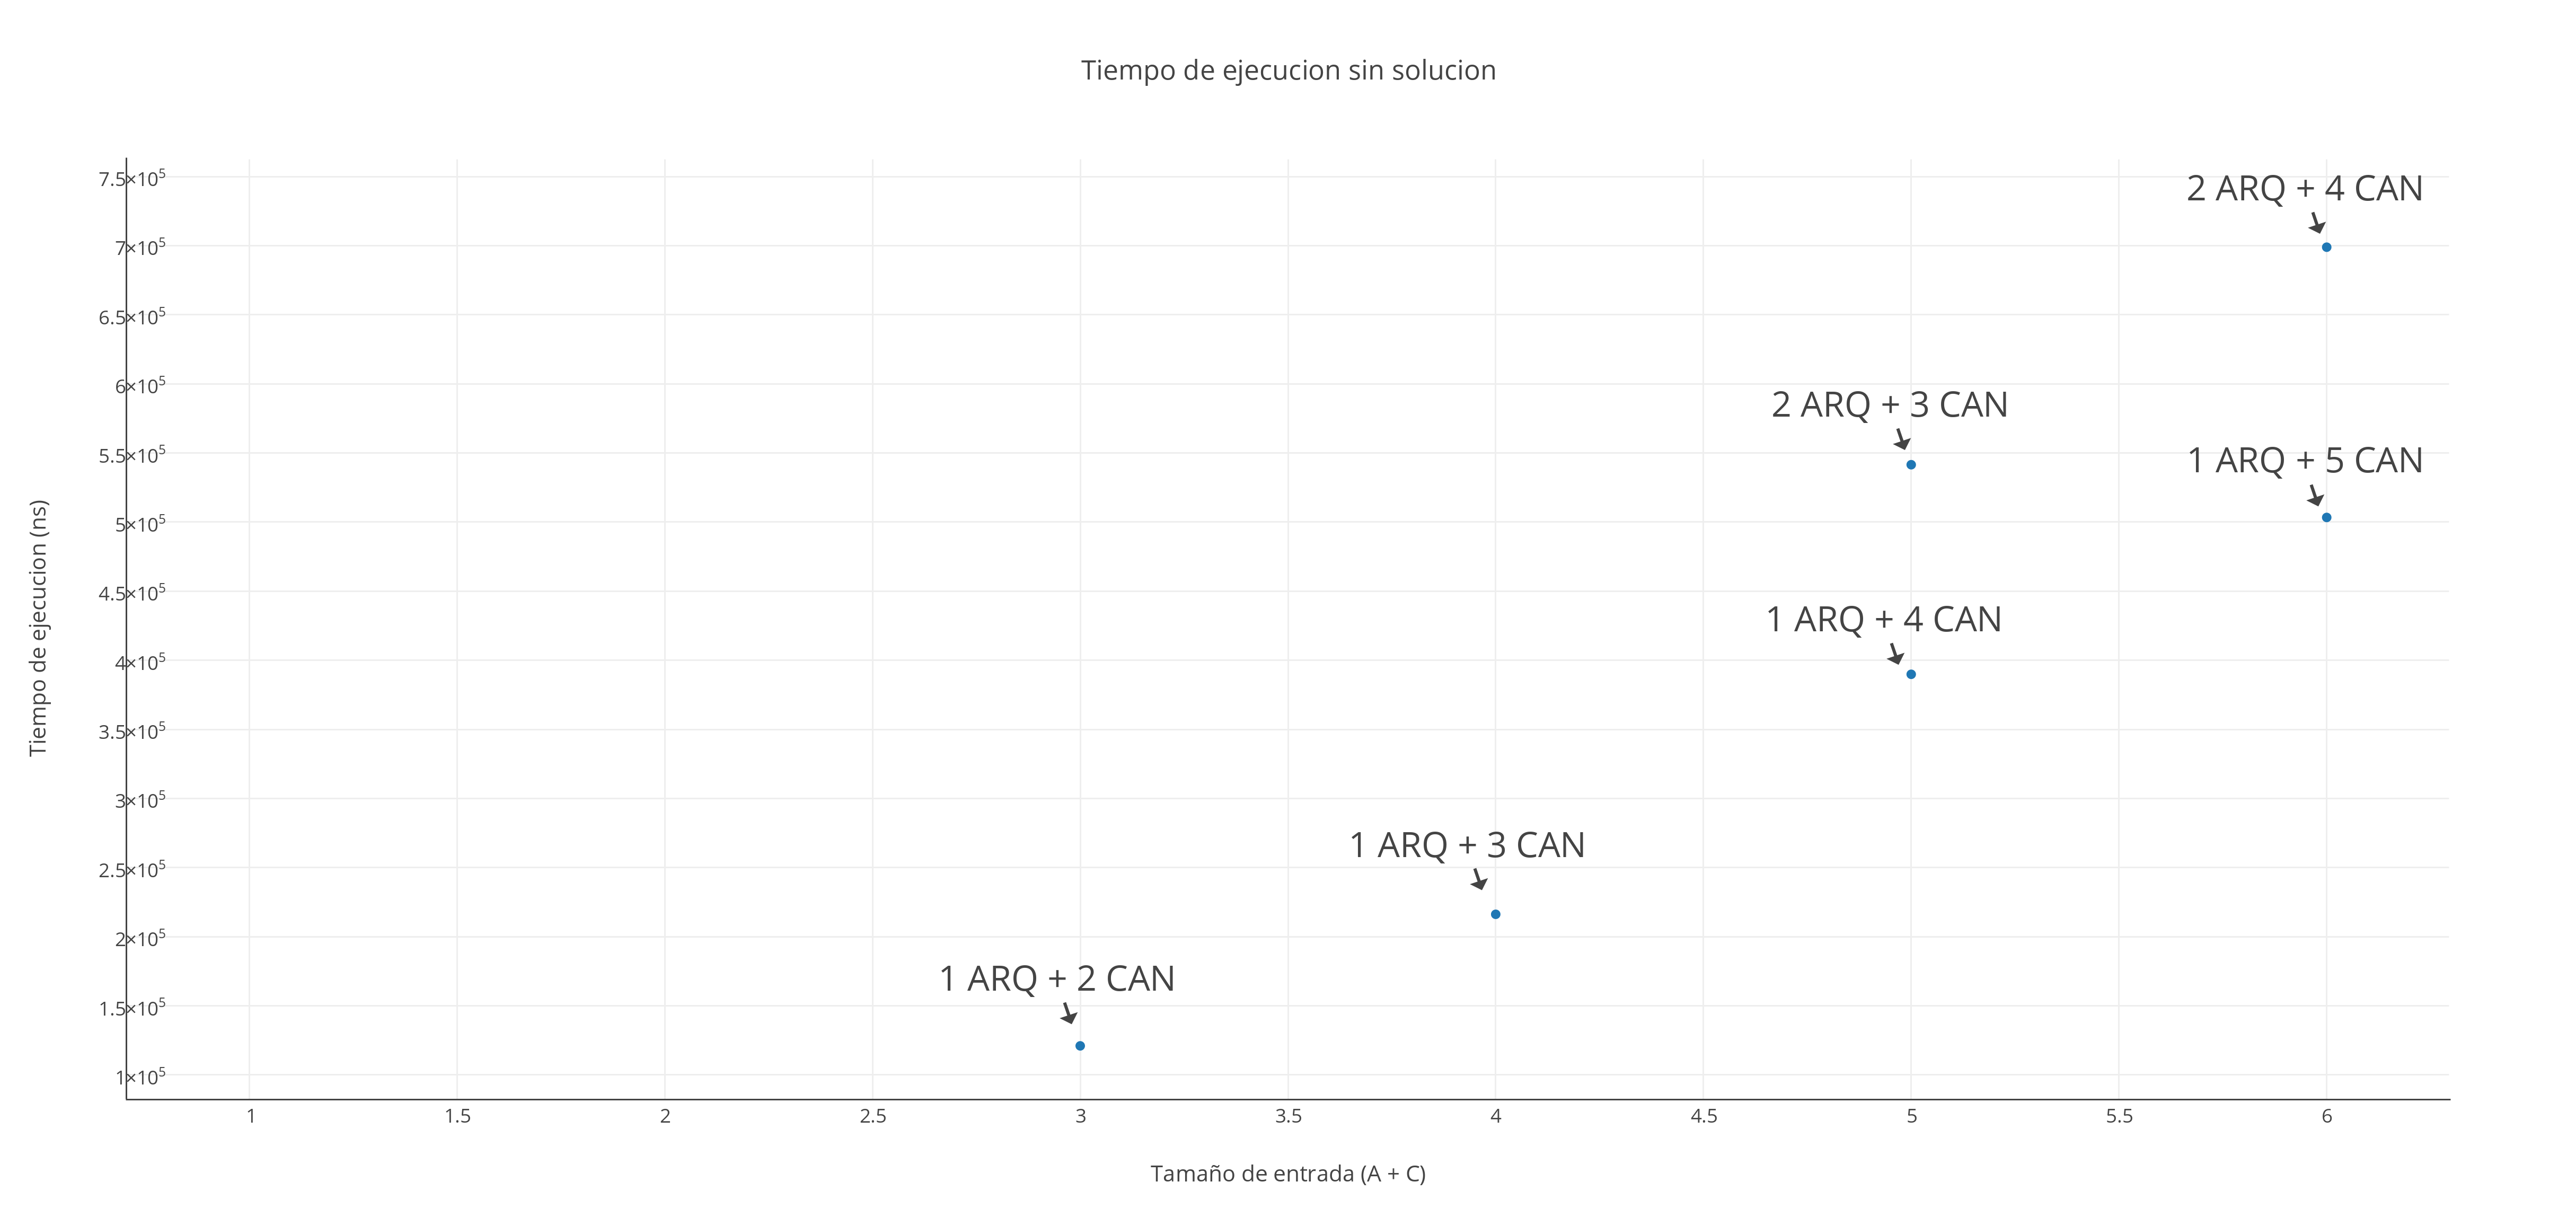
\includegraphics[scale=0.65]{./EJ1/sinsolucion.png}
 {$Gr$\'a$fico$ \ 1.1 - $Sin$ $Solucion$}
  \end{center}
  \vspace*{0.3cm}
 
 \vspace*{0.3cm} \vspace*{0.3cm}
  \begin{center}
 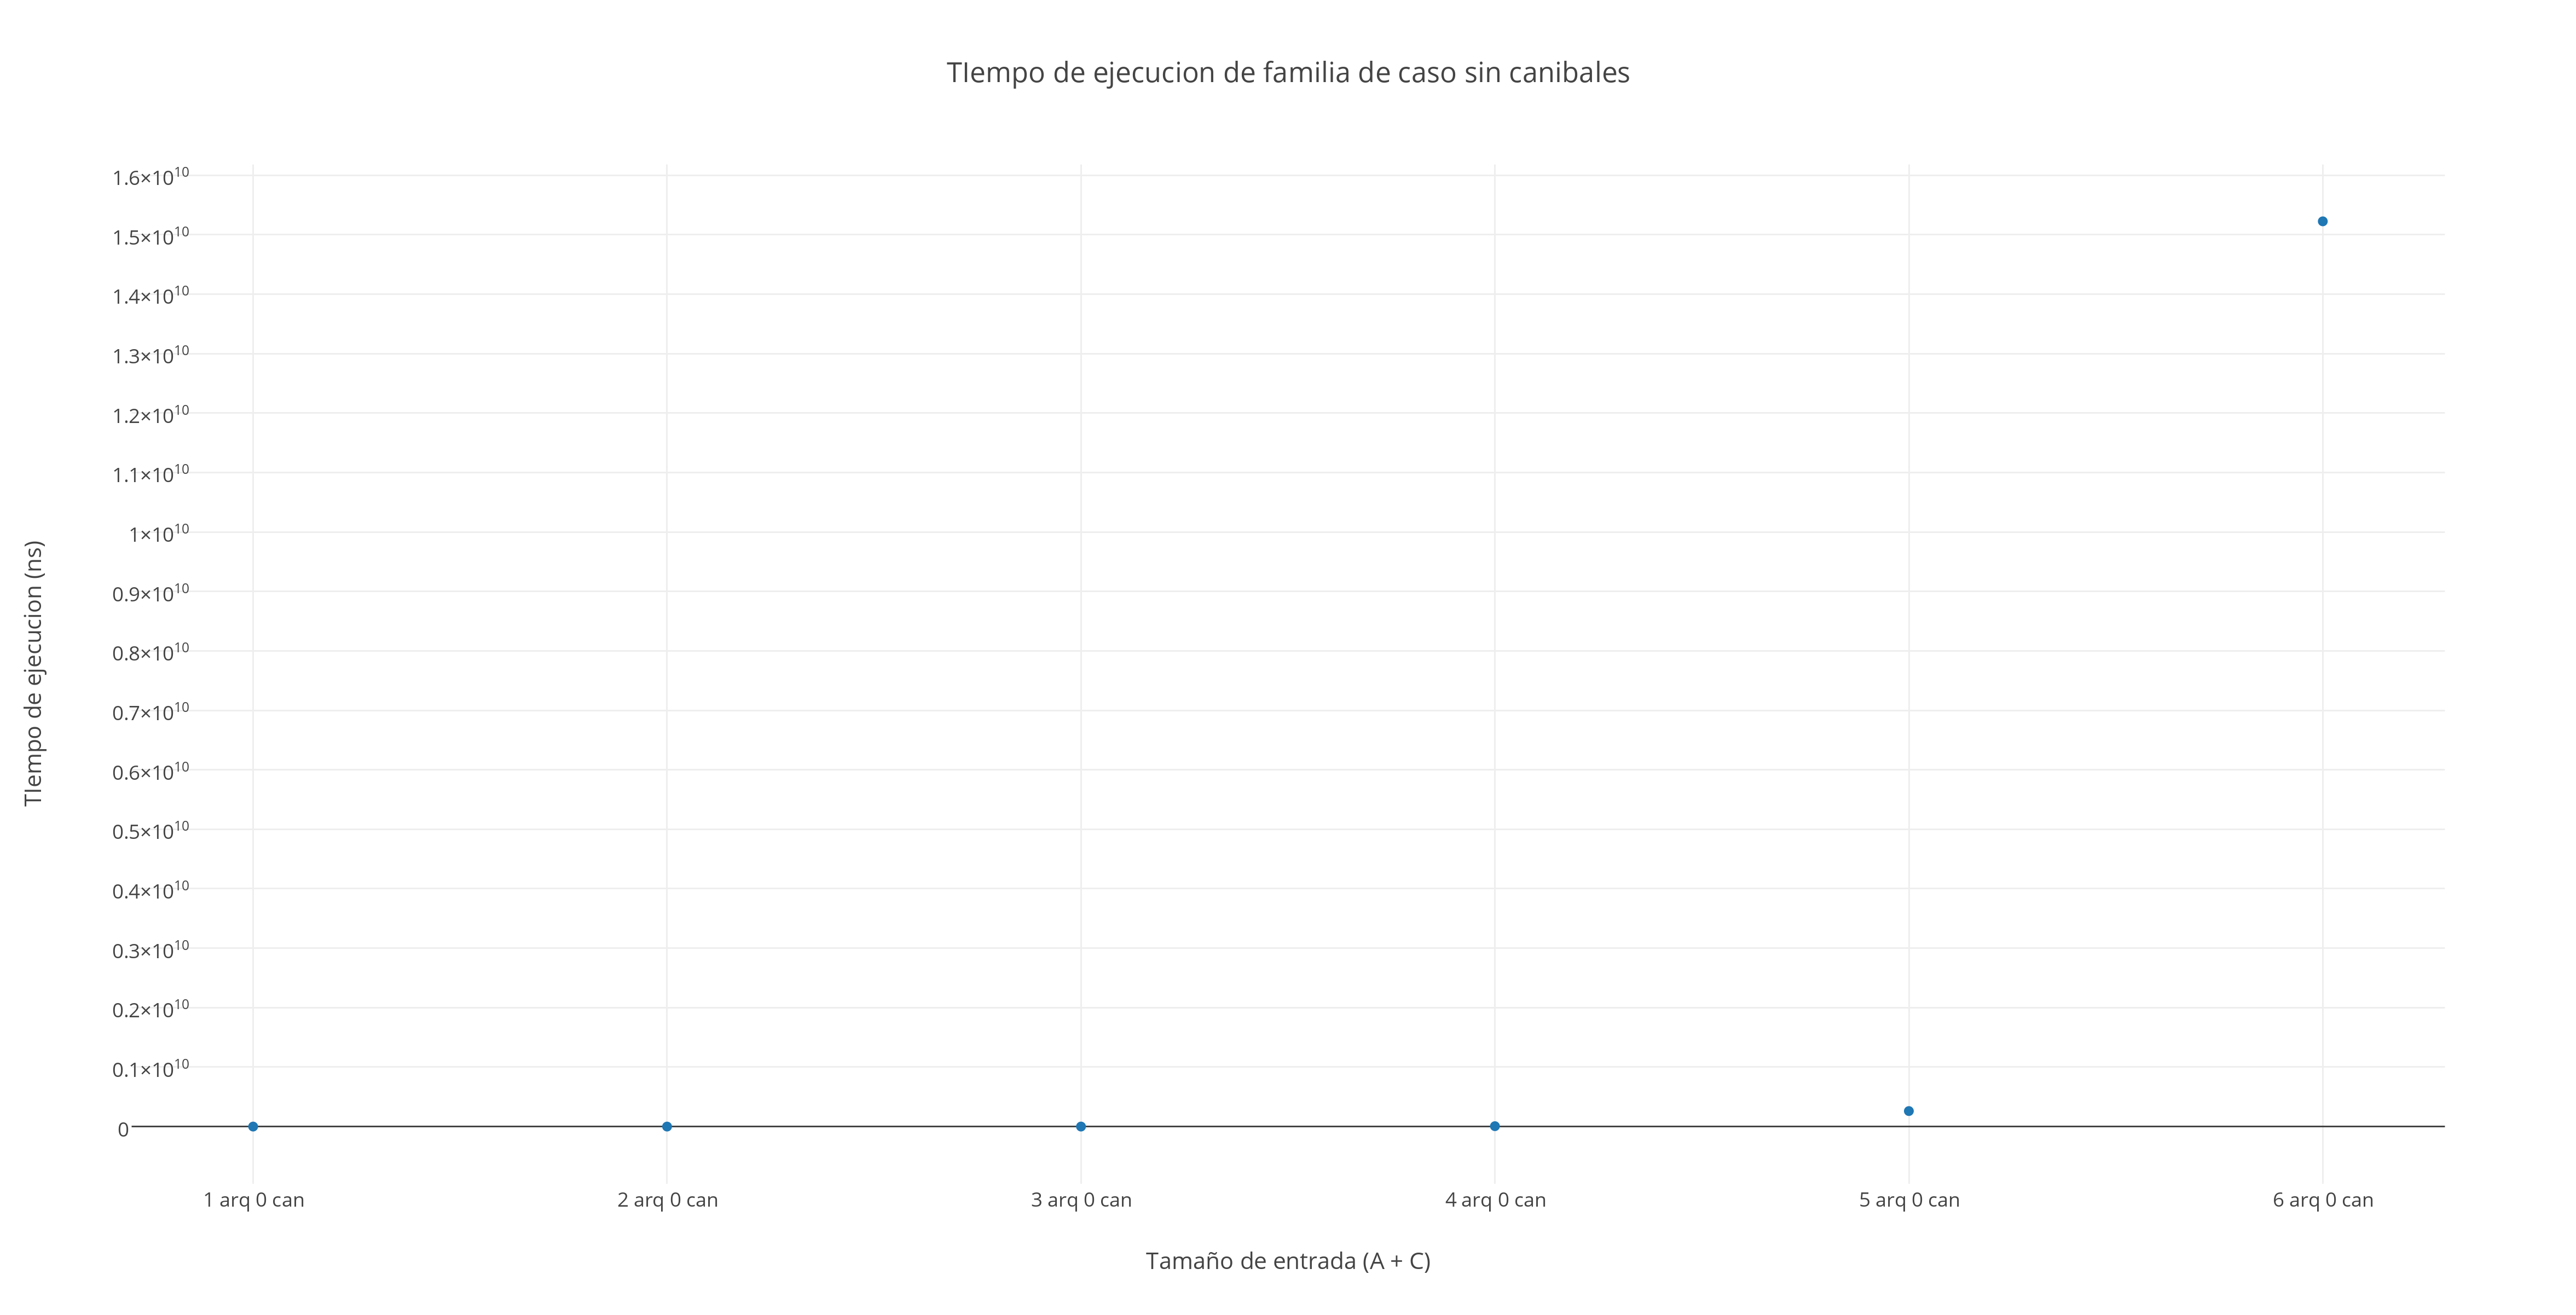
\includegraphics[scale=0.65]{./EJ1/sincanibales.png}
 {$Gr$\'a$fico$ \ 1.2 - $Sin$ $Canibales$}
  \end{center}
  \vspace*{0.3cm}
  
     \vspace*{0.3cm} \vspace*{0.3cm}
  \begin{center}
 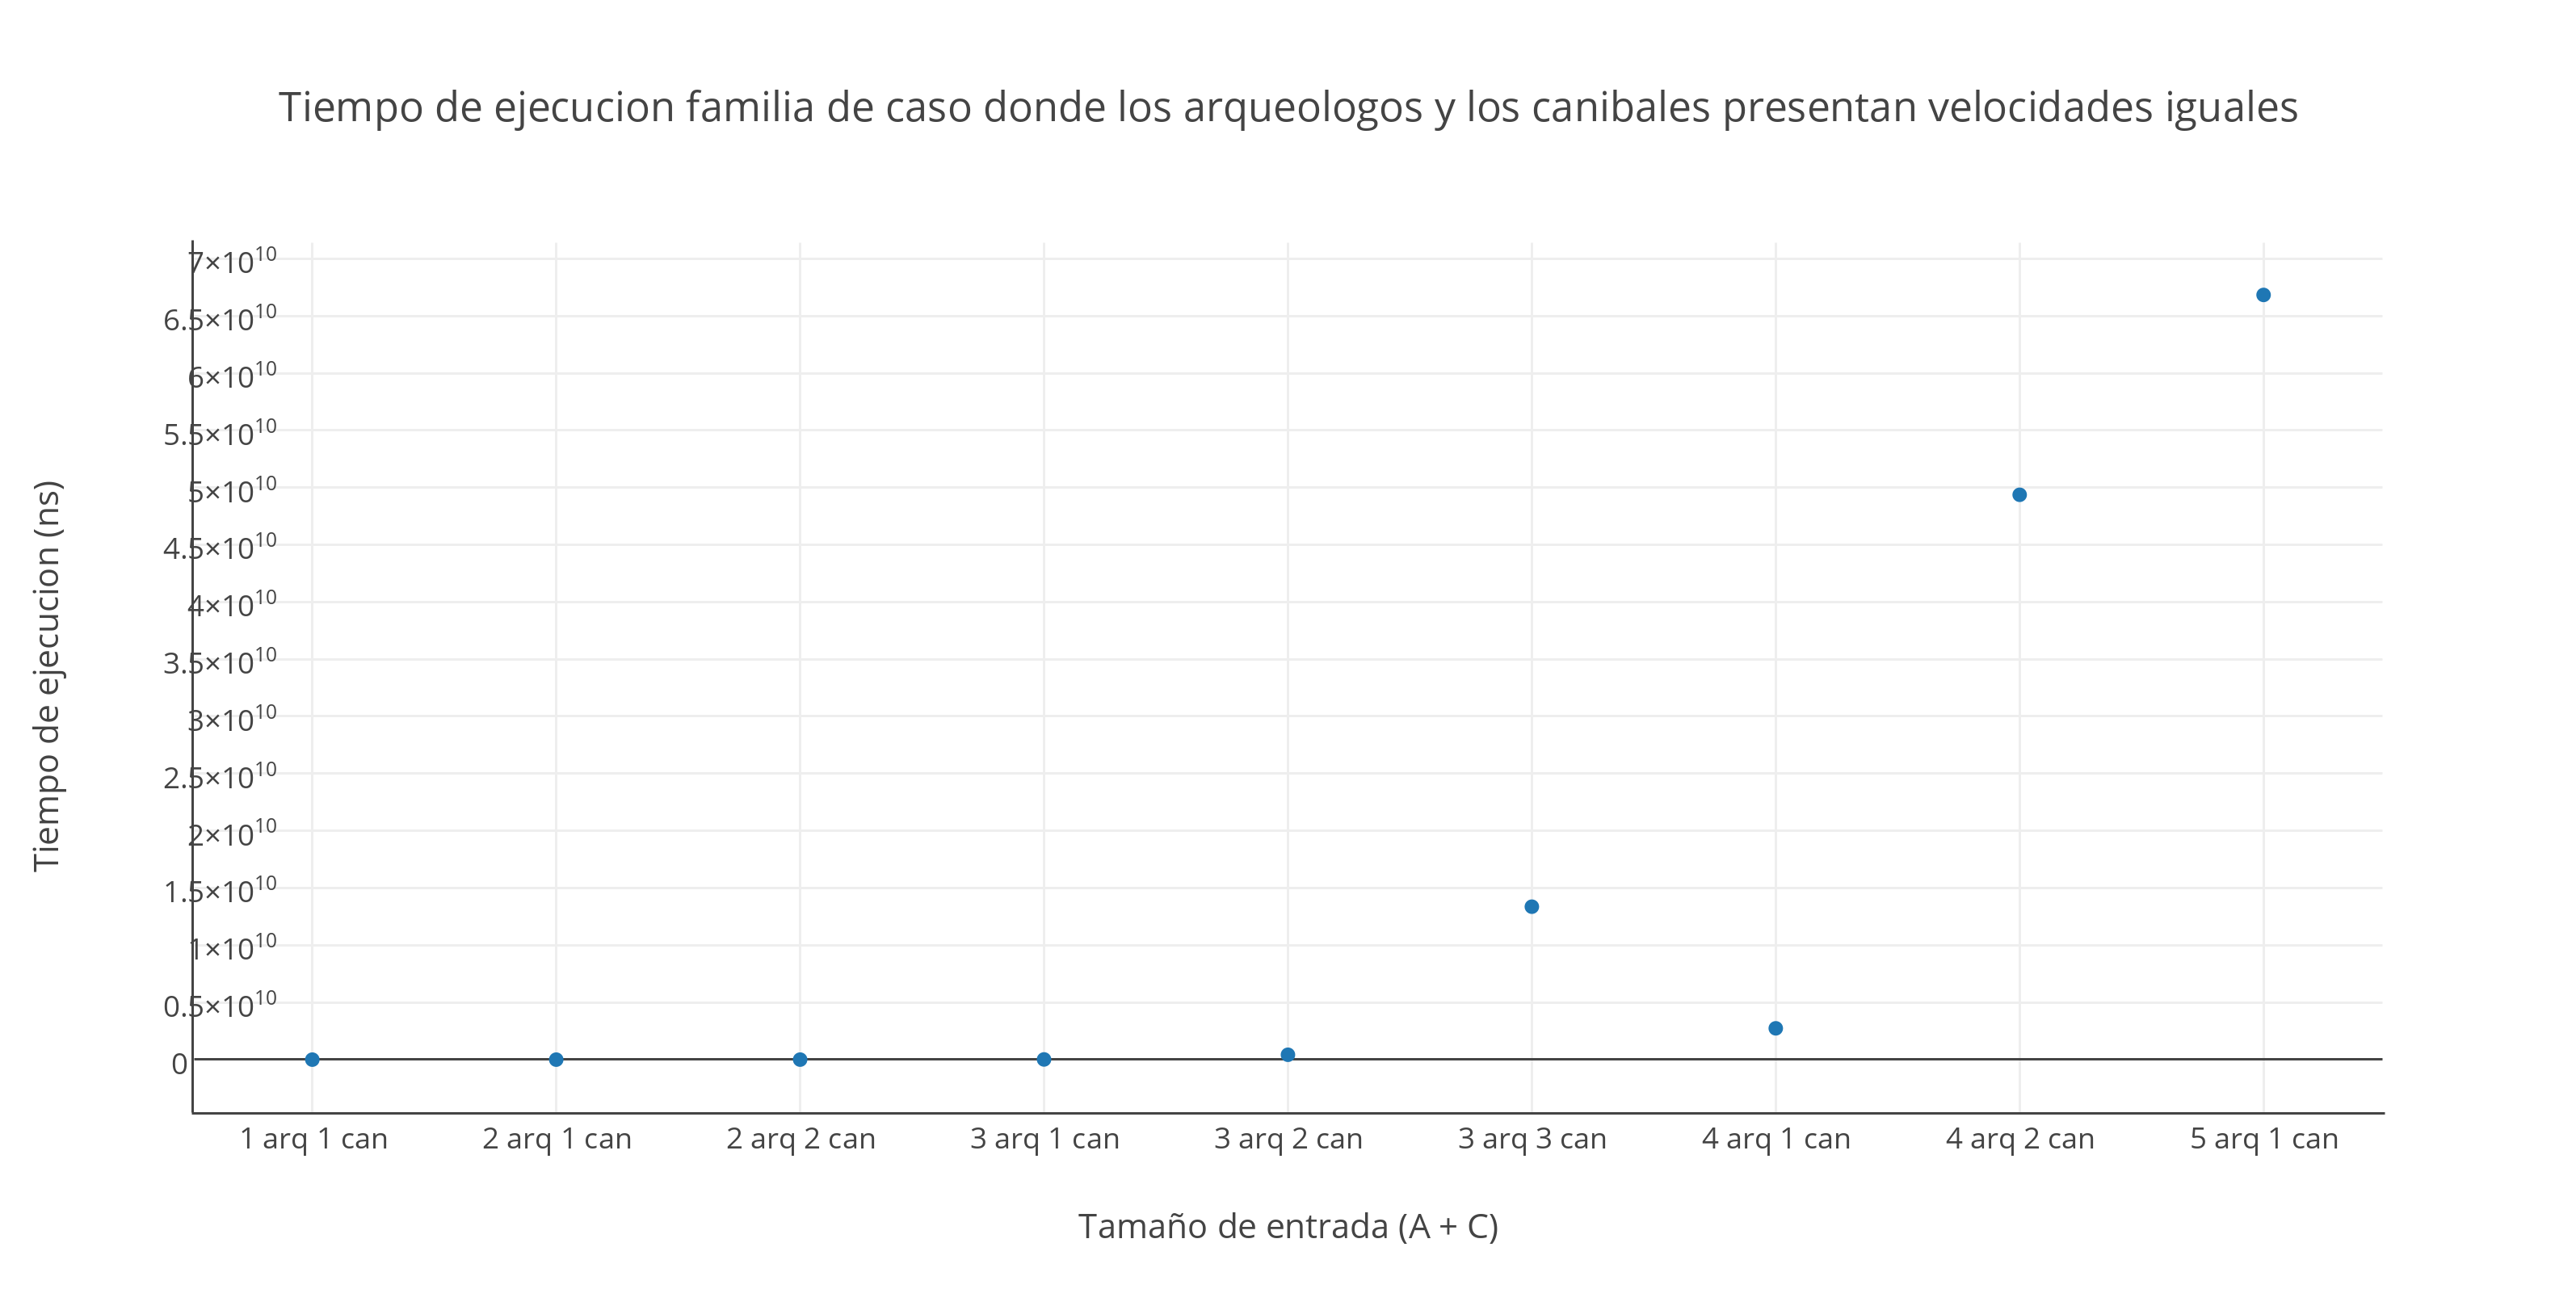
\includegraphics[scale=0.65]{./EJ1/velIgual.png}
 {$Gr$\'a$fico$ \ 1.3 - $Velocidades$ $Iguales$ $Para$ $Todos$}
  \end{center}
  \vspace*{0.3cm}
  
   \vspace*{0.3cm} \vspace*{0.3cm}
  \begin{center}
 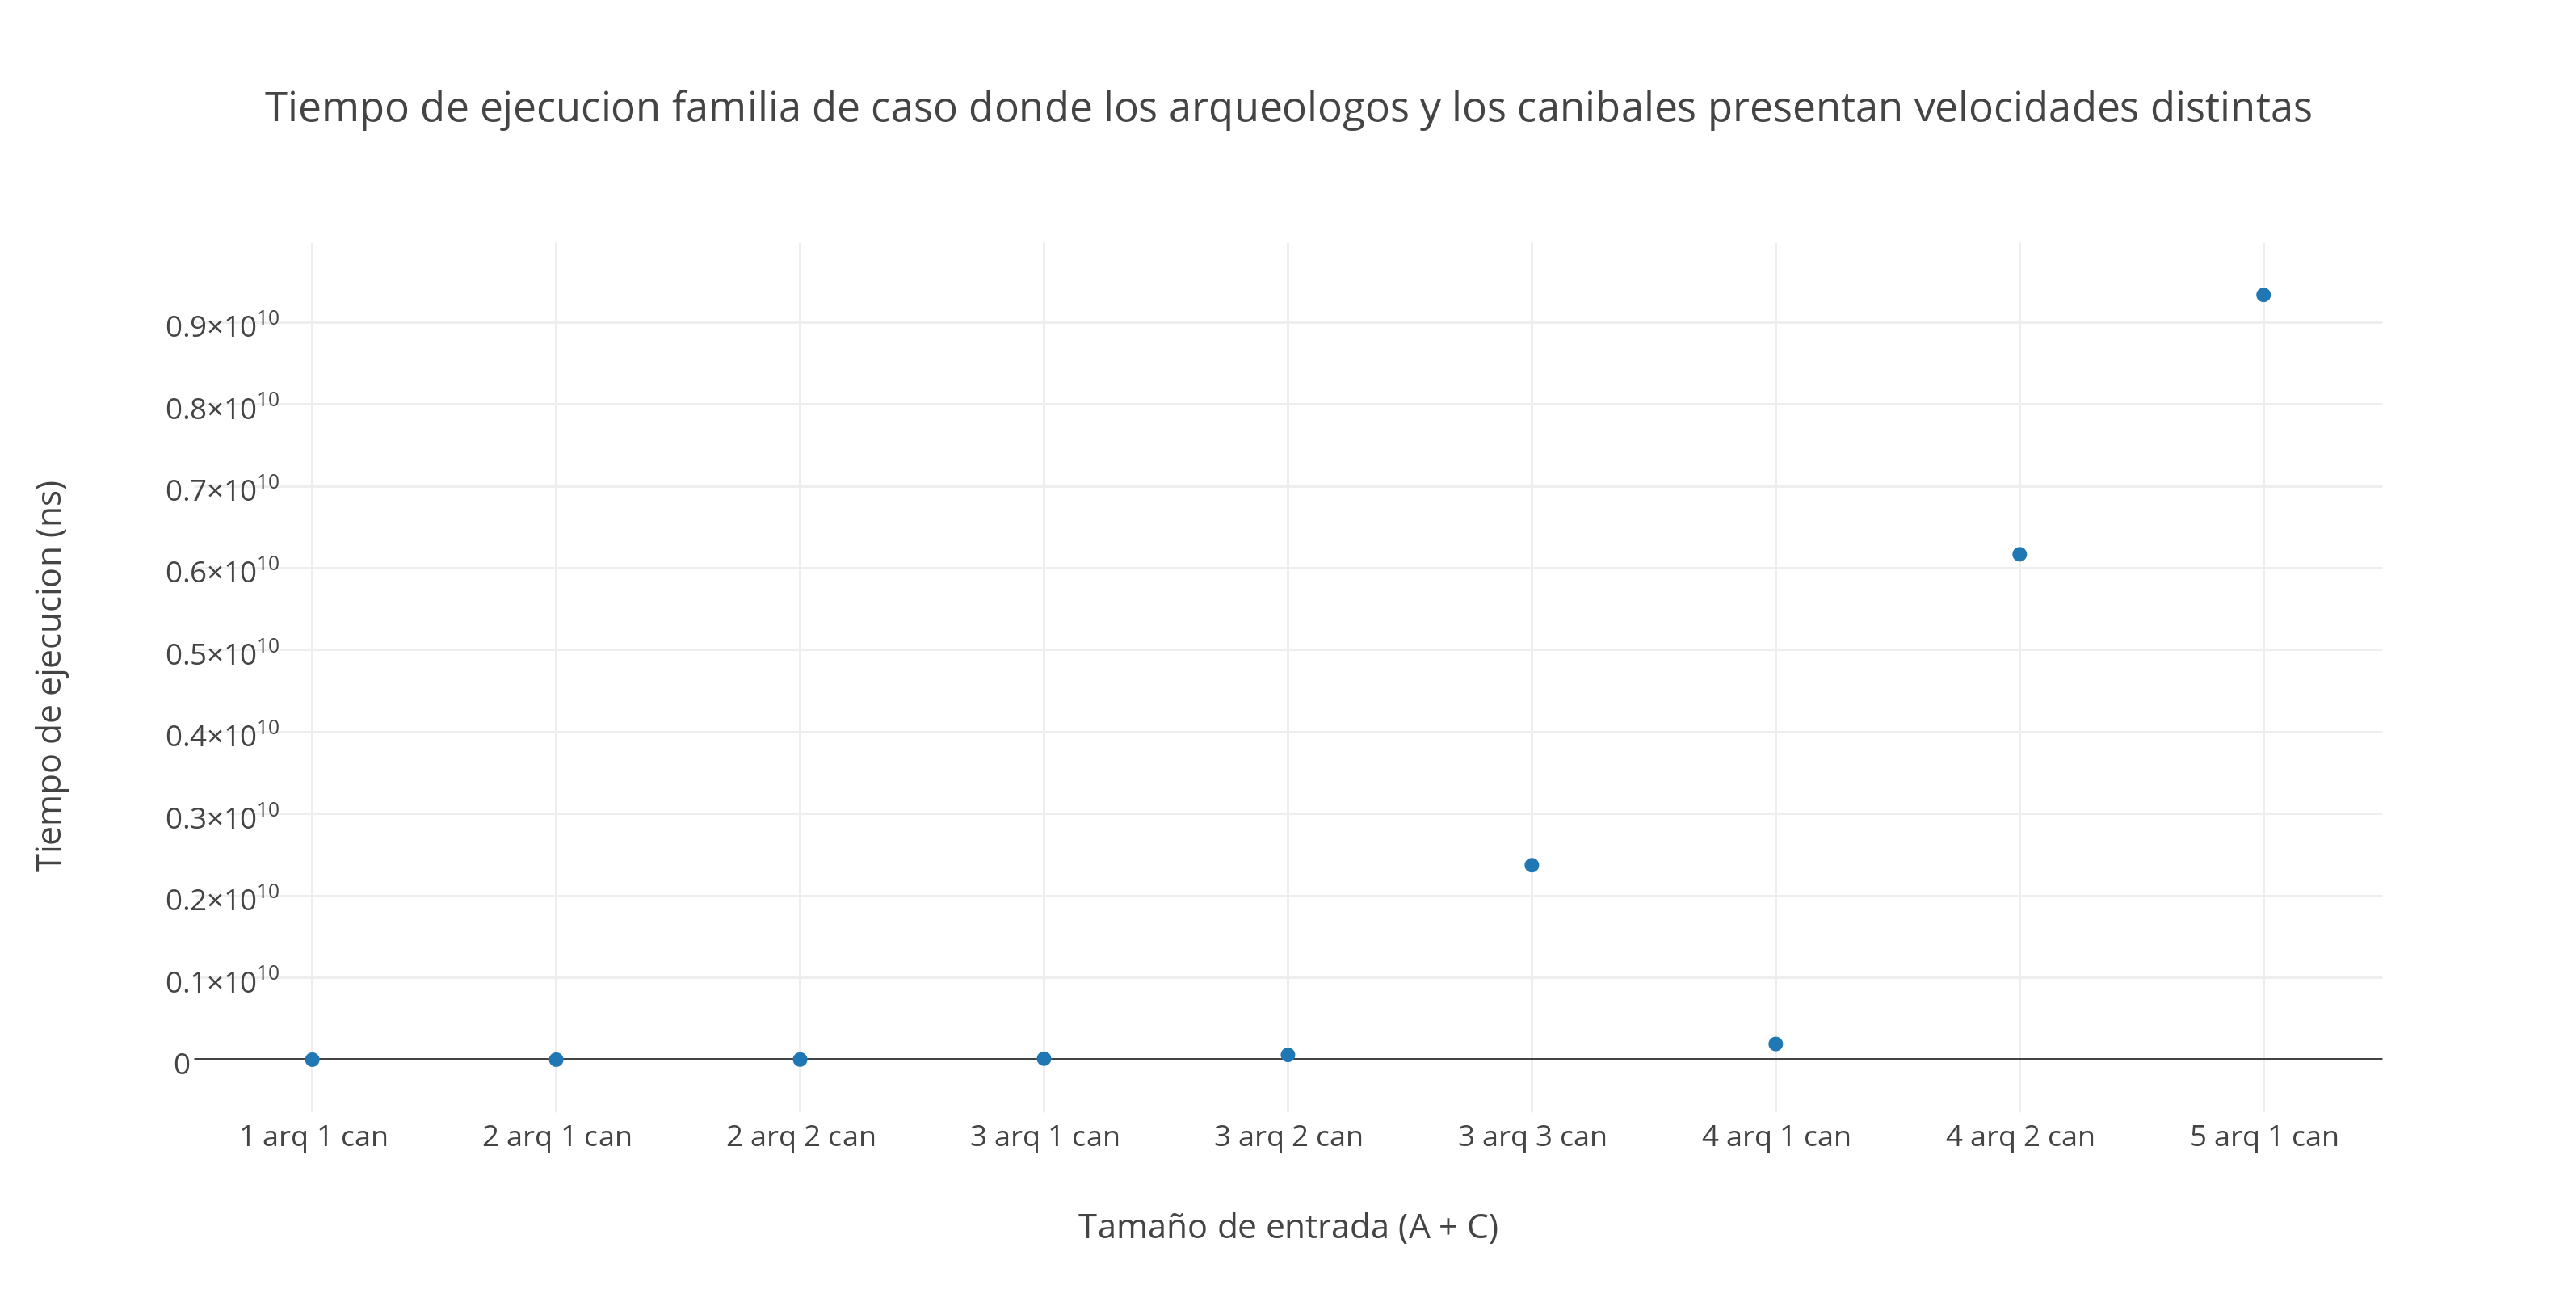
\includegraphics[scale=0.65]{./EJ1/velDistinta.png}
 {$Gr$\'a$fico$ \ 1.4 - $Velocidades$ $Distintas$ $Para$ $Todos$}
  \end{center}
  \vspace*{0.3cm}
  
  
   \vspace*{0.3cm} \vspace*{0.3cm}
  \begin{center}
 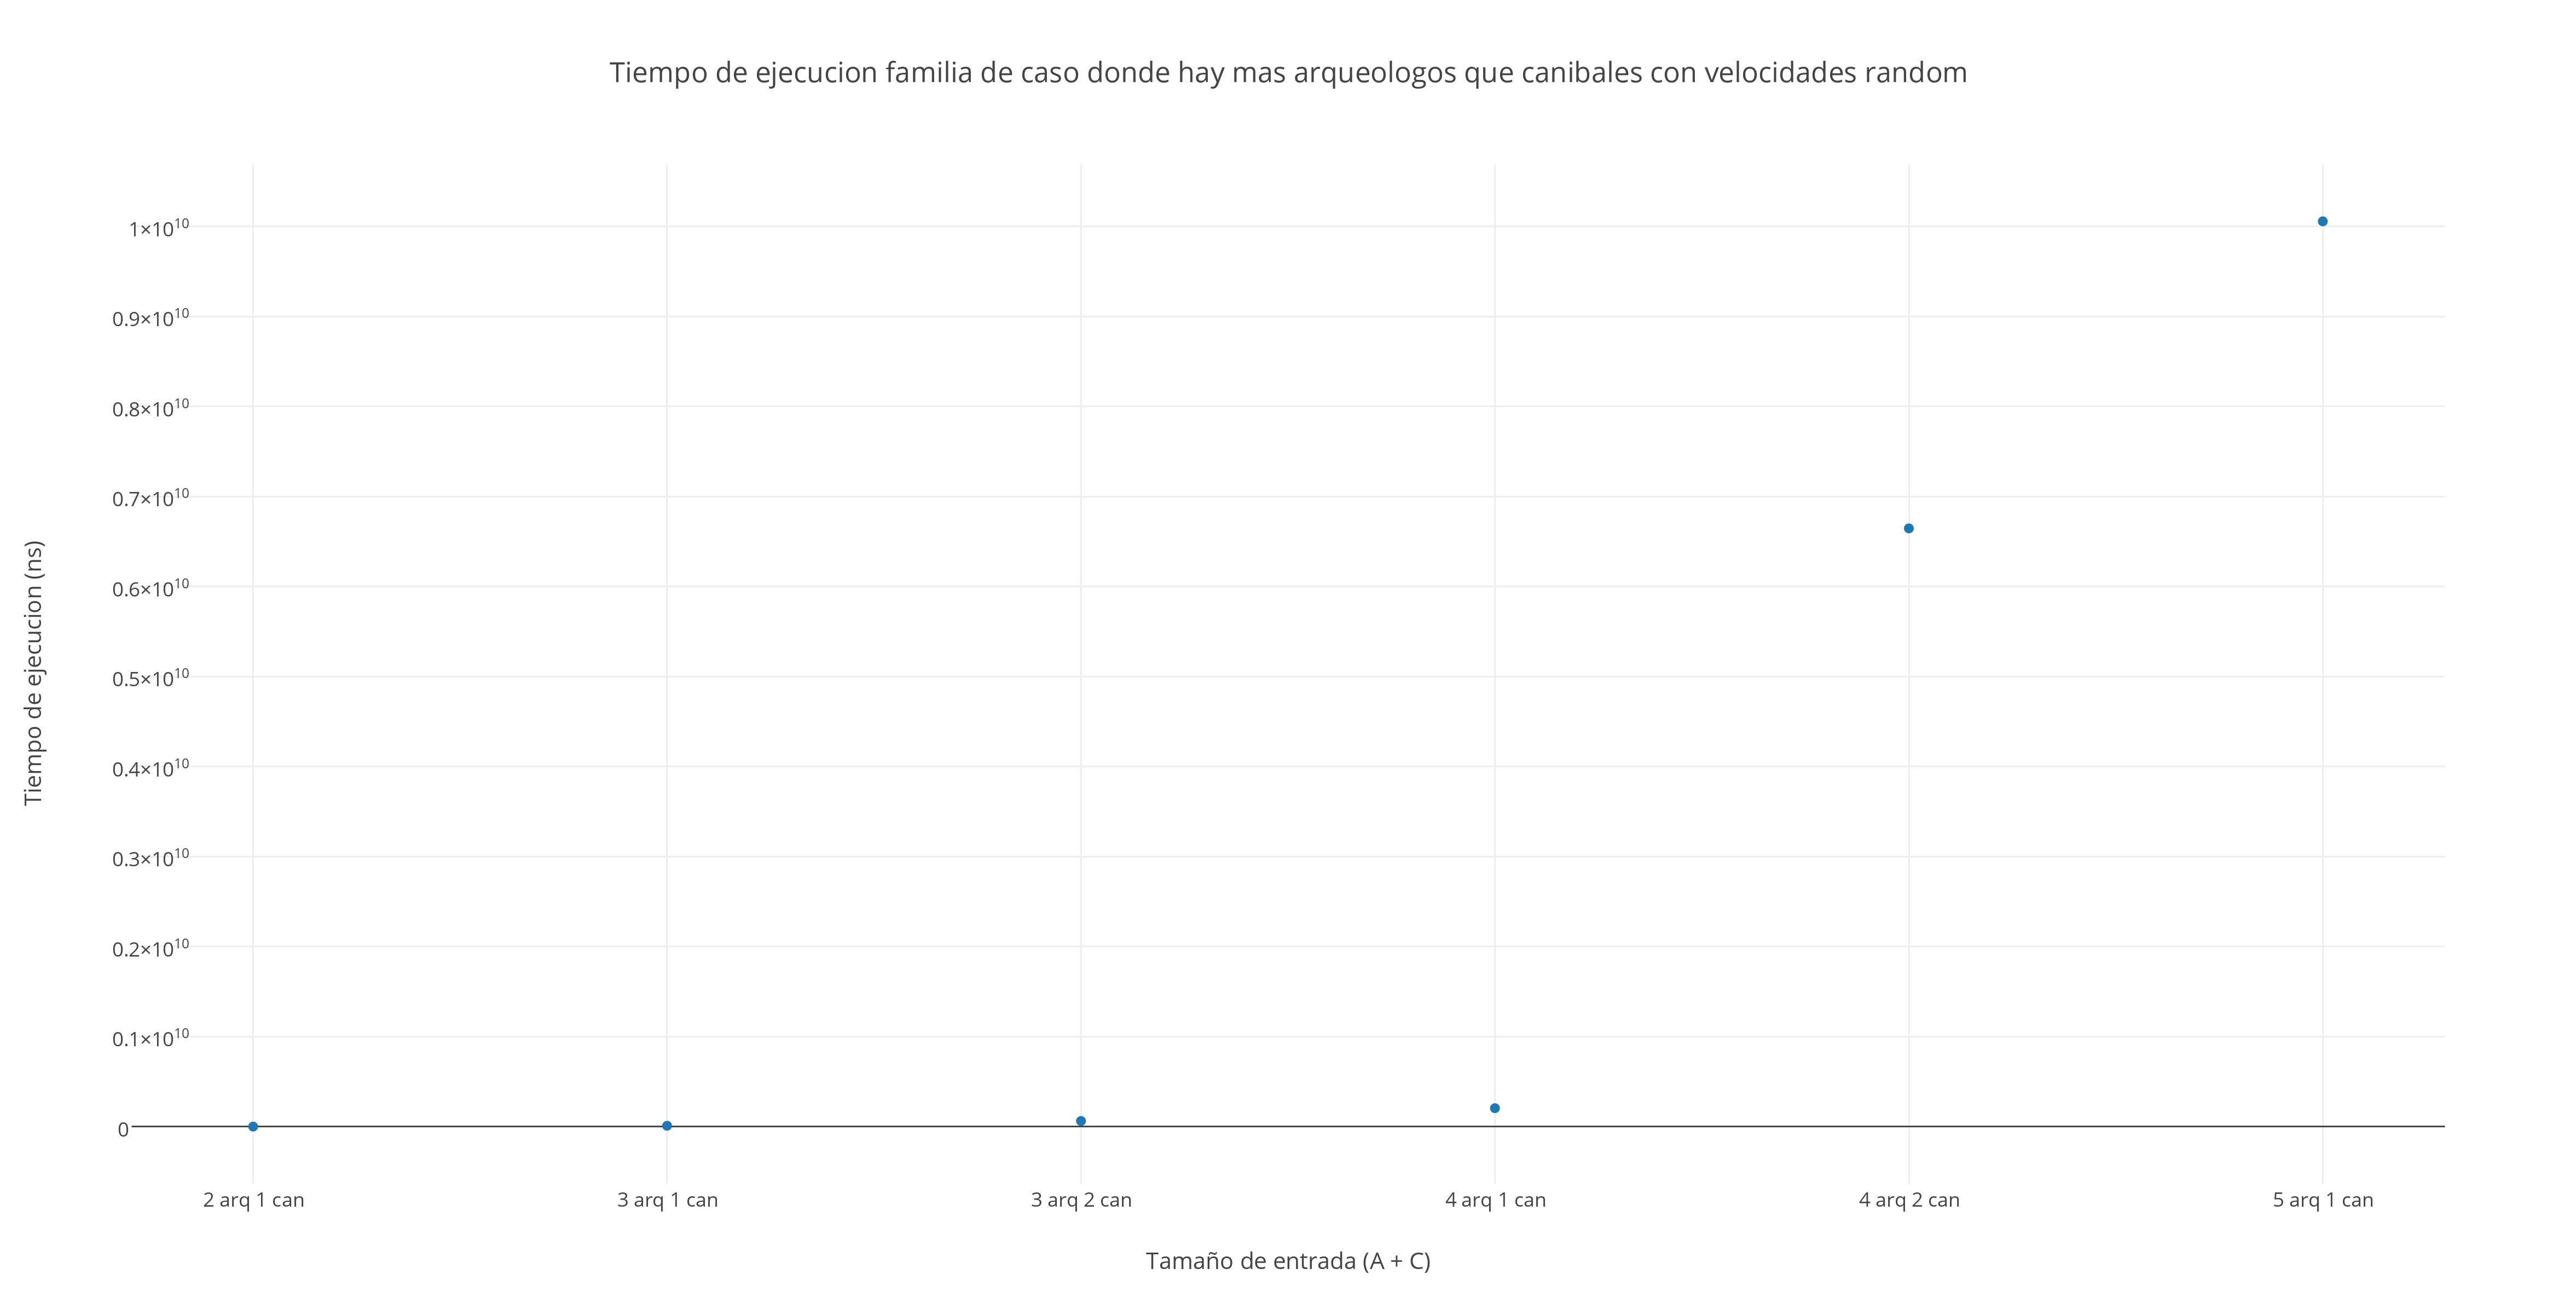
\includegraphics[scale=0.65]{./EJ1/velrandom.png}
 {$Gr$\'a$fico$ \ 1.5 - $Velocidades$ $Random$ $Para$ $Todos$}
  \end{center}
  \vspace*{0.3cm}
  
Luego de realizar dichas mediciones pudimos observar que para los casos en los cuales no hay soluci\'on o no hay canibales se obtiene una mejor performance que para aquellos en los cuales hay soluci\'on siempre y/o hay canibales siempre como son los casos de velocidades distintas o iguales. \\
Es por esto que desarrollamos dos gr\'aficos comparativos para visualizar cual ser\'a nuestro mejor y peor caso.

En el primero trabajaremos con los que se obtiene una mejor performance. Cabe aclarar que debido a que las entradas para un caso no son compatibles en otros (por ejemplo, el caso sin soluci\'on contra el sin canibales), trabajamos con el valor de N final, el cual se obtiene de sumar la cantidad de arqueologos con la cantidad de canibales.\\

   \vspace*{0.3cm} \vspace*{0.3cm}
  \begin{center}
 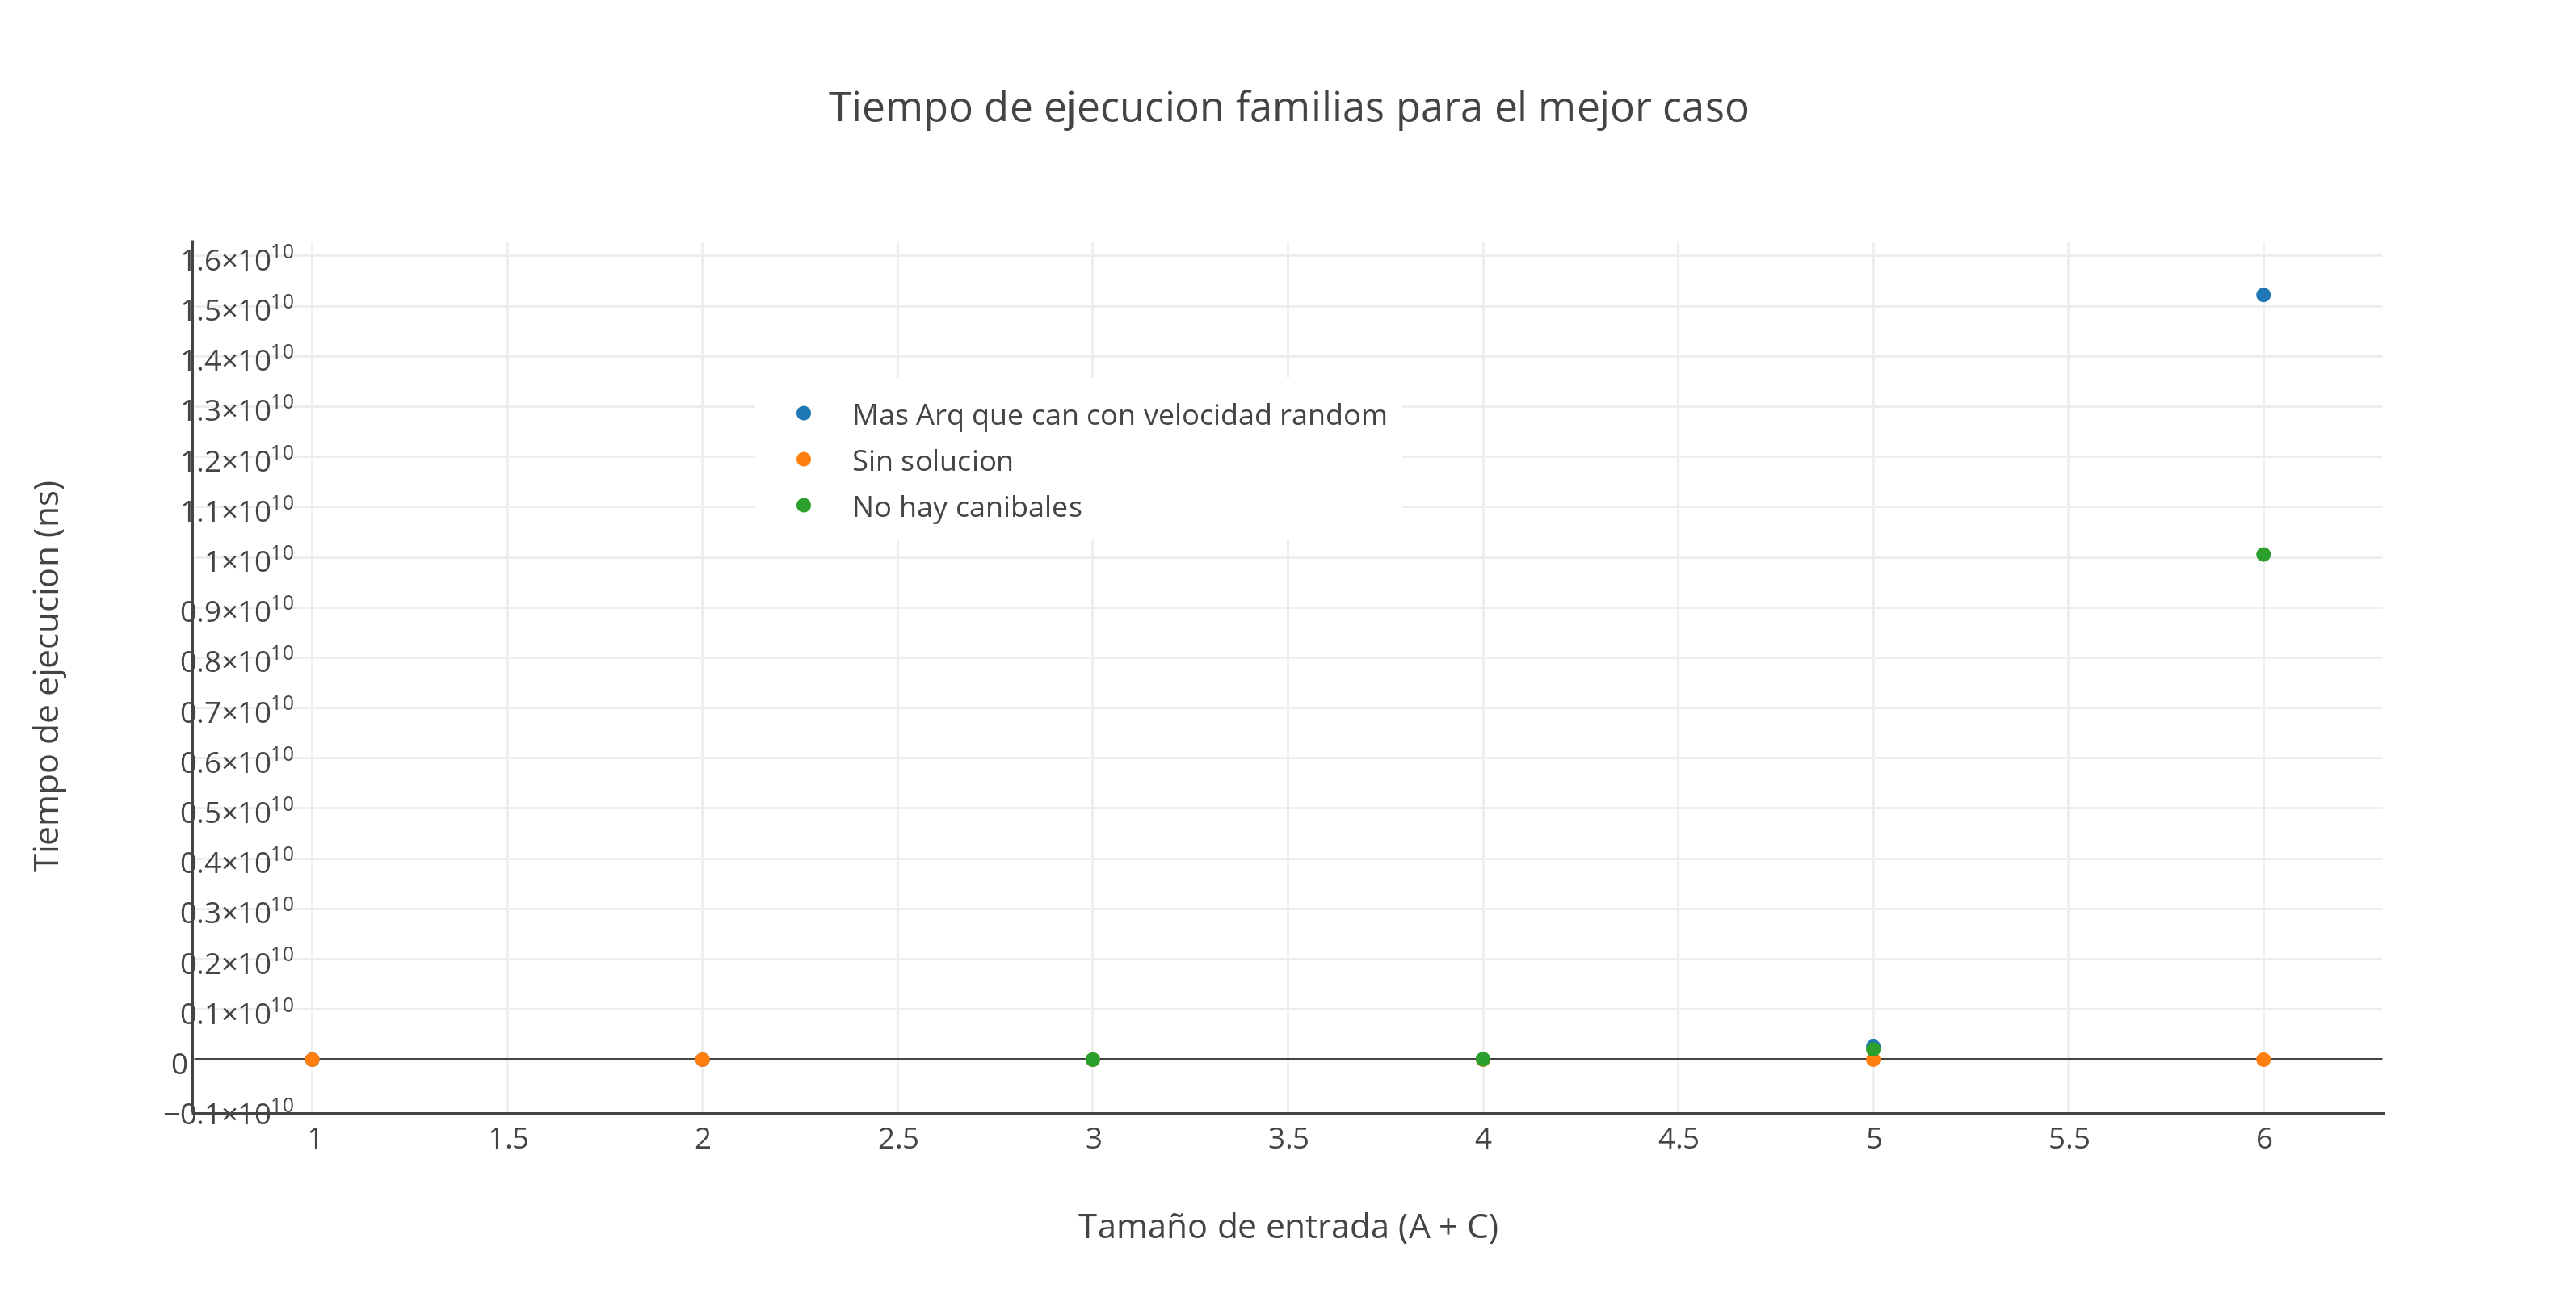
\includegraphics[scale=0.65]{./EJ1/comparativomejorcaso.png}
 {$Gr$\'a$fico$ \ 1.6 - $Comparativo$ $Mejor$ $Caso$}
  \end{center}
  \vspace*{0.3cm}

Se puede observar en el gr\'afico, tres funciones las cuales representan el tiempo de ejecuci\'on de las familias que resultan mas beneficiadas al trabajar con nuestro algoritmo:\\
\begin{itemize}
\item Hay m\'as canibales que arqueologos, es decir, no hay soluci\'on.
\item No hay canibales
\item Hay m\'as arqueologos que canibales con velocidades dispares
\end{itemize}

Como se observa en el gr\'afico la funci\'on representativa de la flia n\'umero 1, presenta una mejor performance en relaci\'on a las otras. Esto se debe a que nuestro algoritmo como  va chequeando y probando todos los posibles pares que viajen de un lado al otro, y, como inicialmente chequea que hay m\'as canibales que arqueologos imposibilitando un par posible, el algoritmo corta sin probar los posibles pares, finalizando su ejecuci\'on.

Luego de haber chequeado dichas instancias, pudimos llegar a la conclusi\'on que la familia de casos que presenta una mejor performance para nuestro algoritmo
es en el cual \textbf{Hay m\'as canibales que arqueologos, es decir, no hay soluci\'on}

Para una mayor observaci\'on desarrollamos el siguiente gr\'afico con las instancias:\\

\vspace*{0.3cm} \vspace*{0.3cm}
  \begin{center}
 %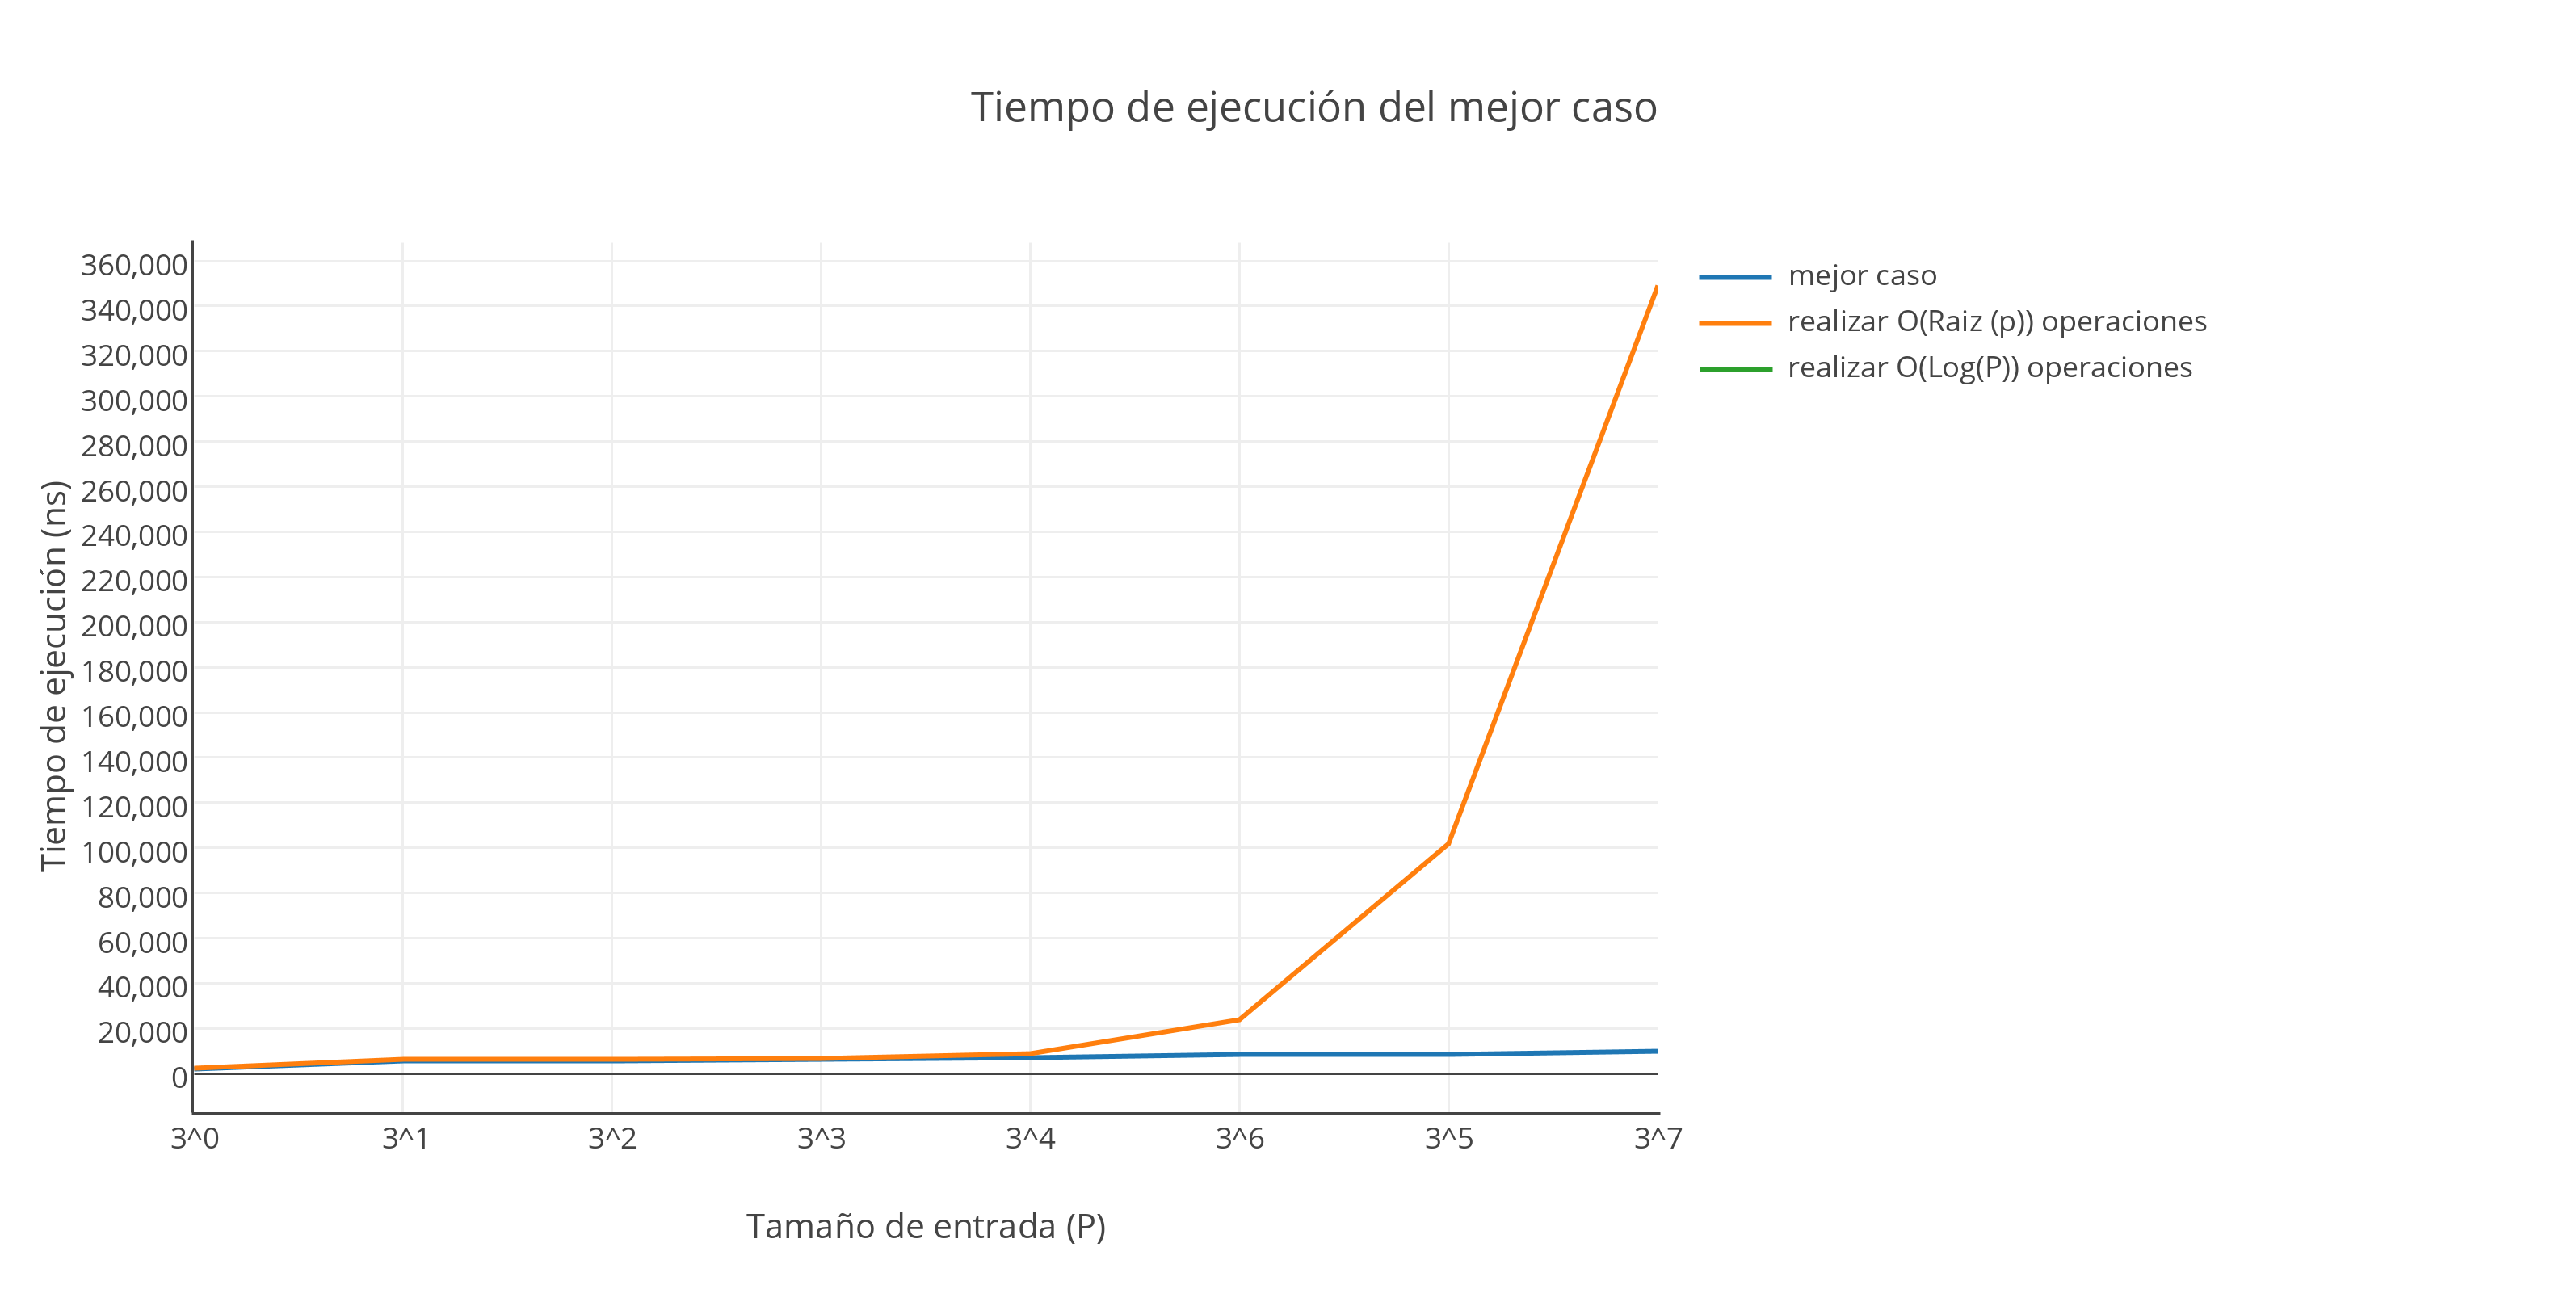
\includegraphics[scale=0.65]{./EJ2/mejorcaso.png}
 {$Gr$\'a$fico$ \ 1.2 - $Mejor Caso$}
  \end{center}
  \vspace*{0.3cm}
  
%Como es posible observar en el gr\'afico, la funci\'on resultante de la cota teorica crece mucho m\'as r\'apido que la de nuestro algoritmo la cual se tiende a ser constante, es por esto que a la hora de realizar el gr\'afico de mediciones se tomaron los primeros valores debido a que, cuando la funci\'on de $\sqrt{P}$ toma valores muy grandes la misma es imposible de graficar contra nuestro algoritmo, por lo cual realizamos un apartado con las instancias m\'as grandes (ver excel).

%Adem\'as, como se puede apreciar debido a lo comentado no es posible apreciar las diferencias entre nuestro algoritmo y la cota O(Log(P)) es por esto que mostraremos un gr\'afico entre ambos:\\

\vspace*{0.3cm} \vspace*{0.3cm}
  \begin{center}
%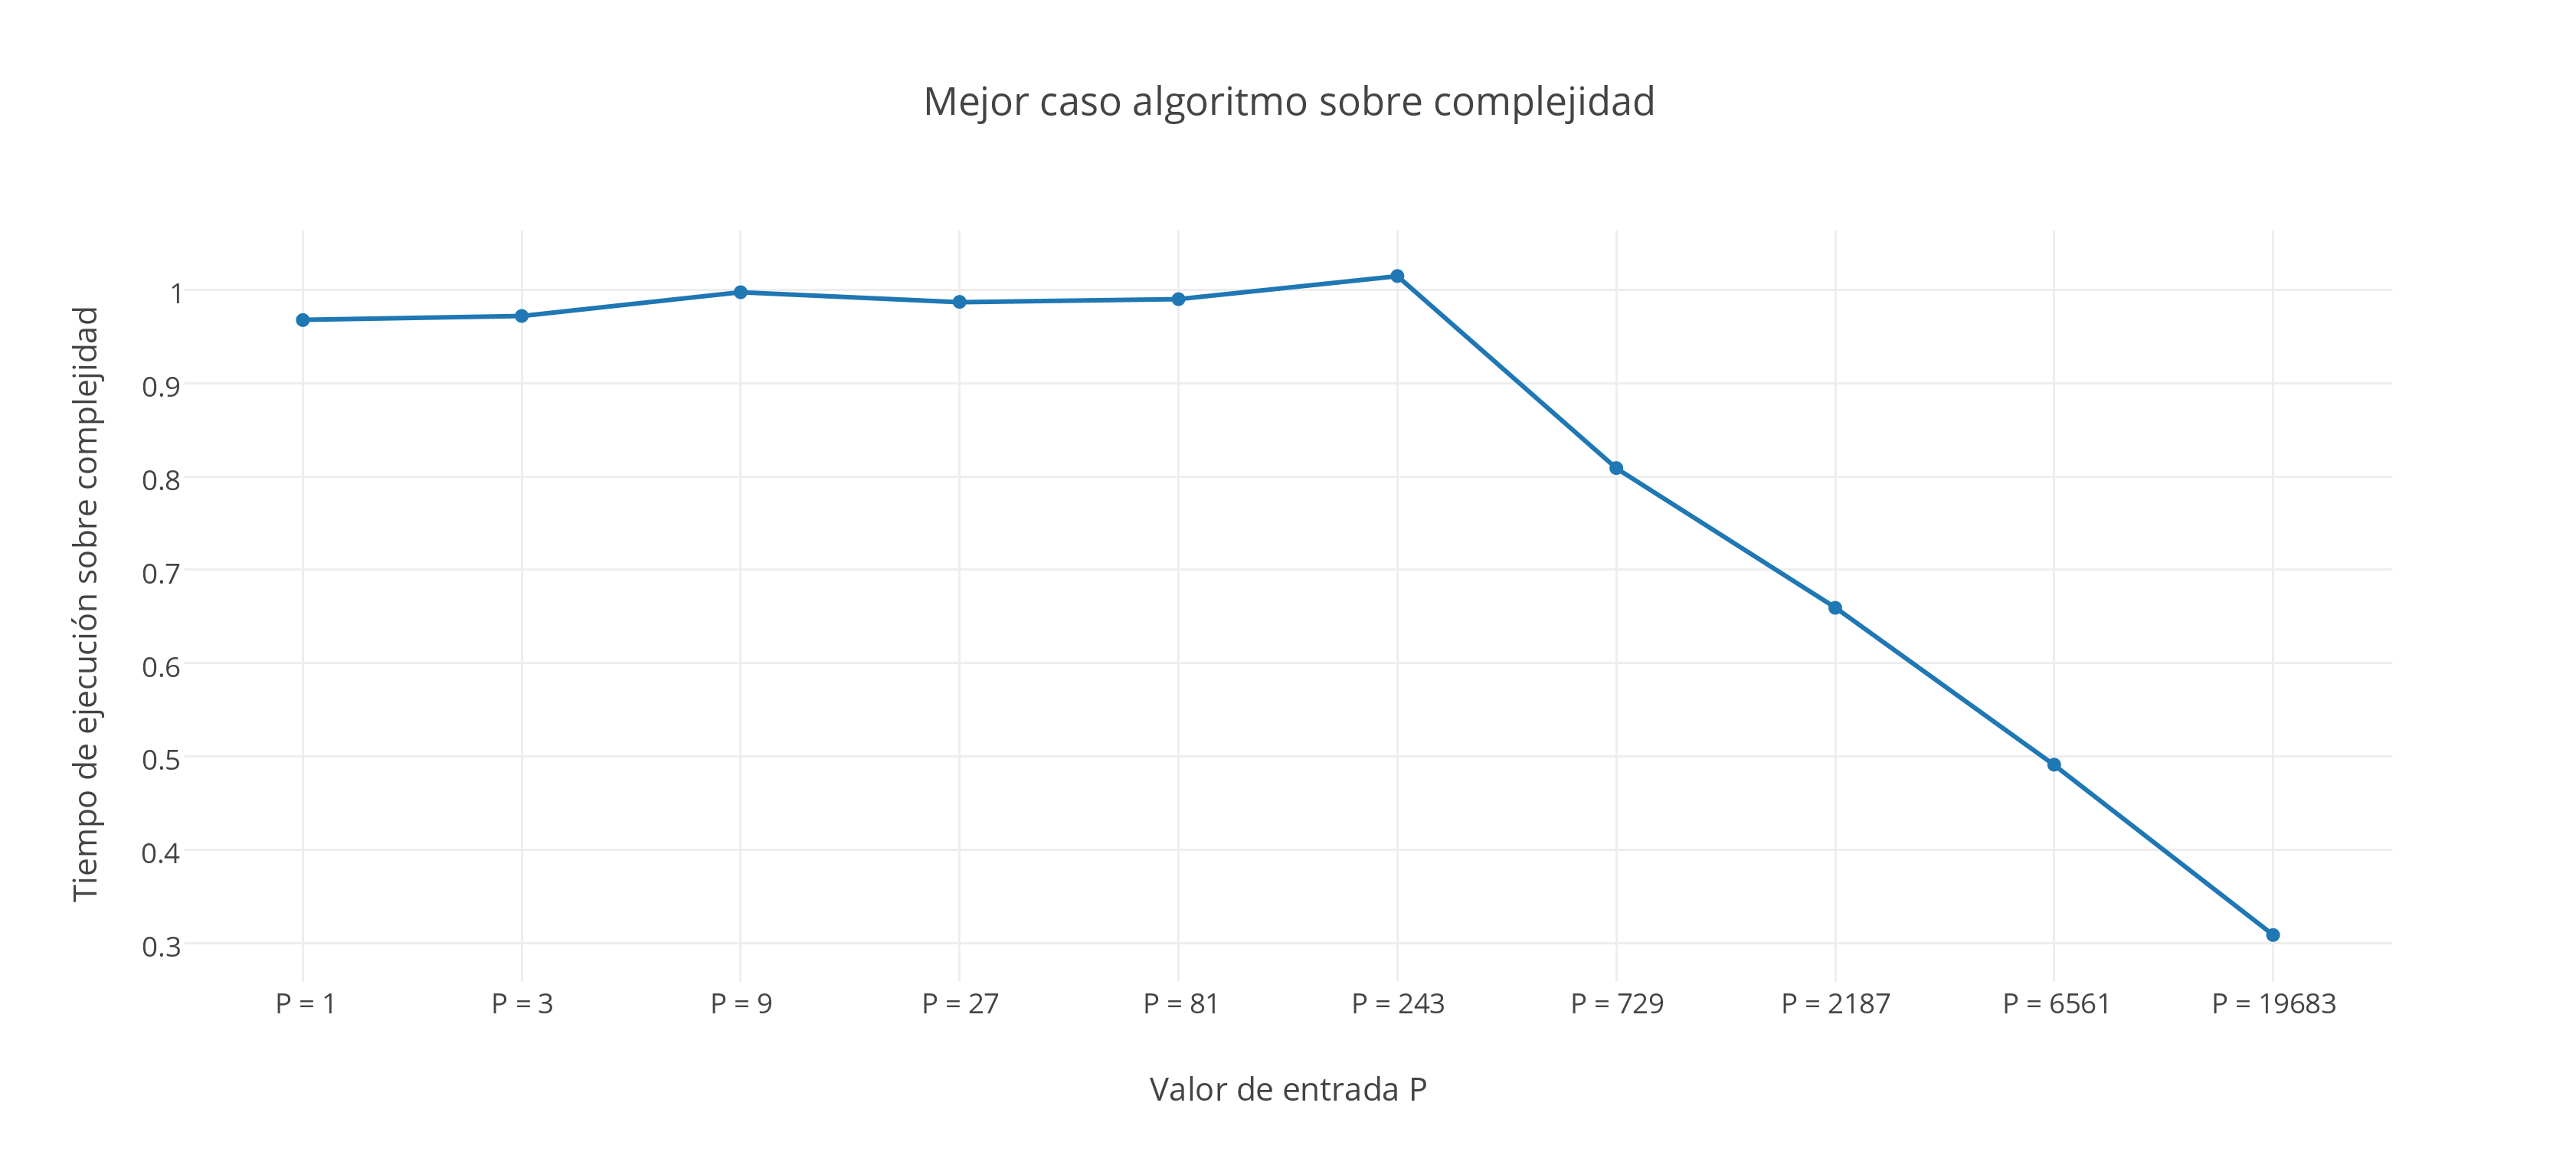
\includegraphics[scale=0.65]{./EJ2/mejorcaso2.png}
{$Gr$\'a$fico$ \ 1.3 - $Mejor Caso$}
  \end{center}
  \vspace*{0.3cm}


Luego, dividiendo por la complejidad teorica de nuestro algoritmo llegamos a:\\

\vspace*{0.3cm} \vspace*{0.3cm}
  \begin{center}
%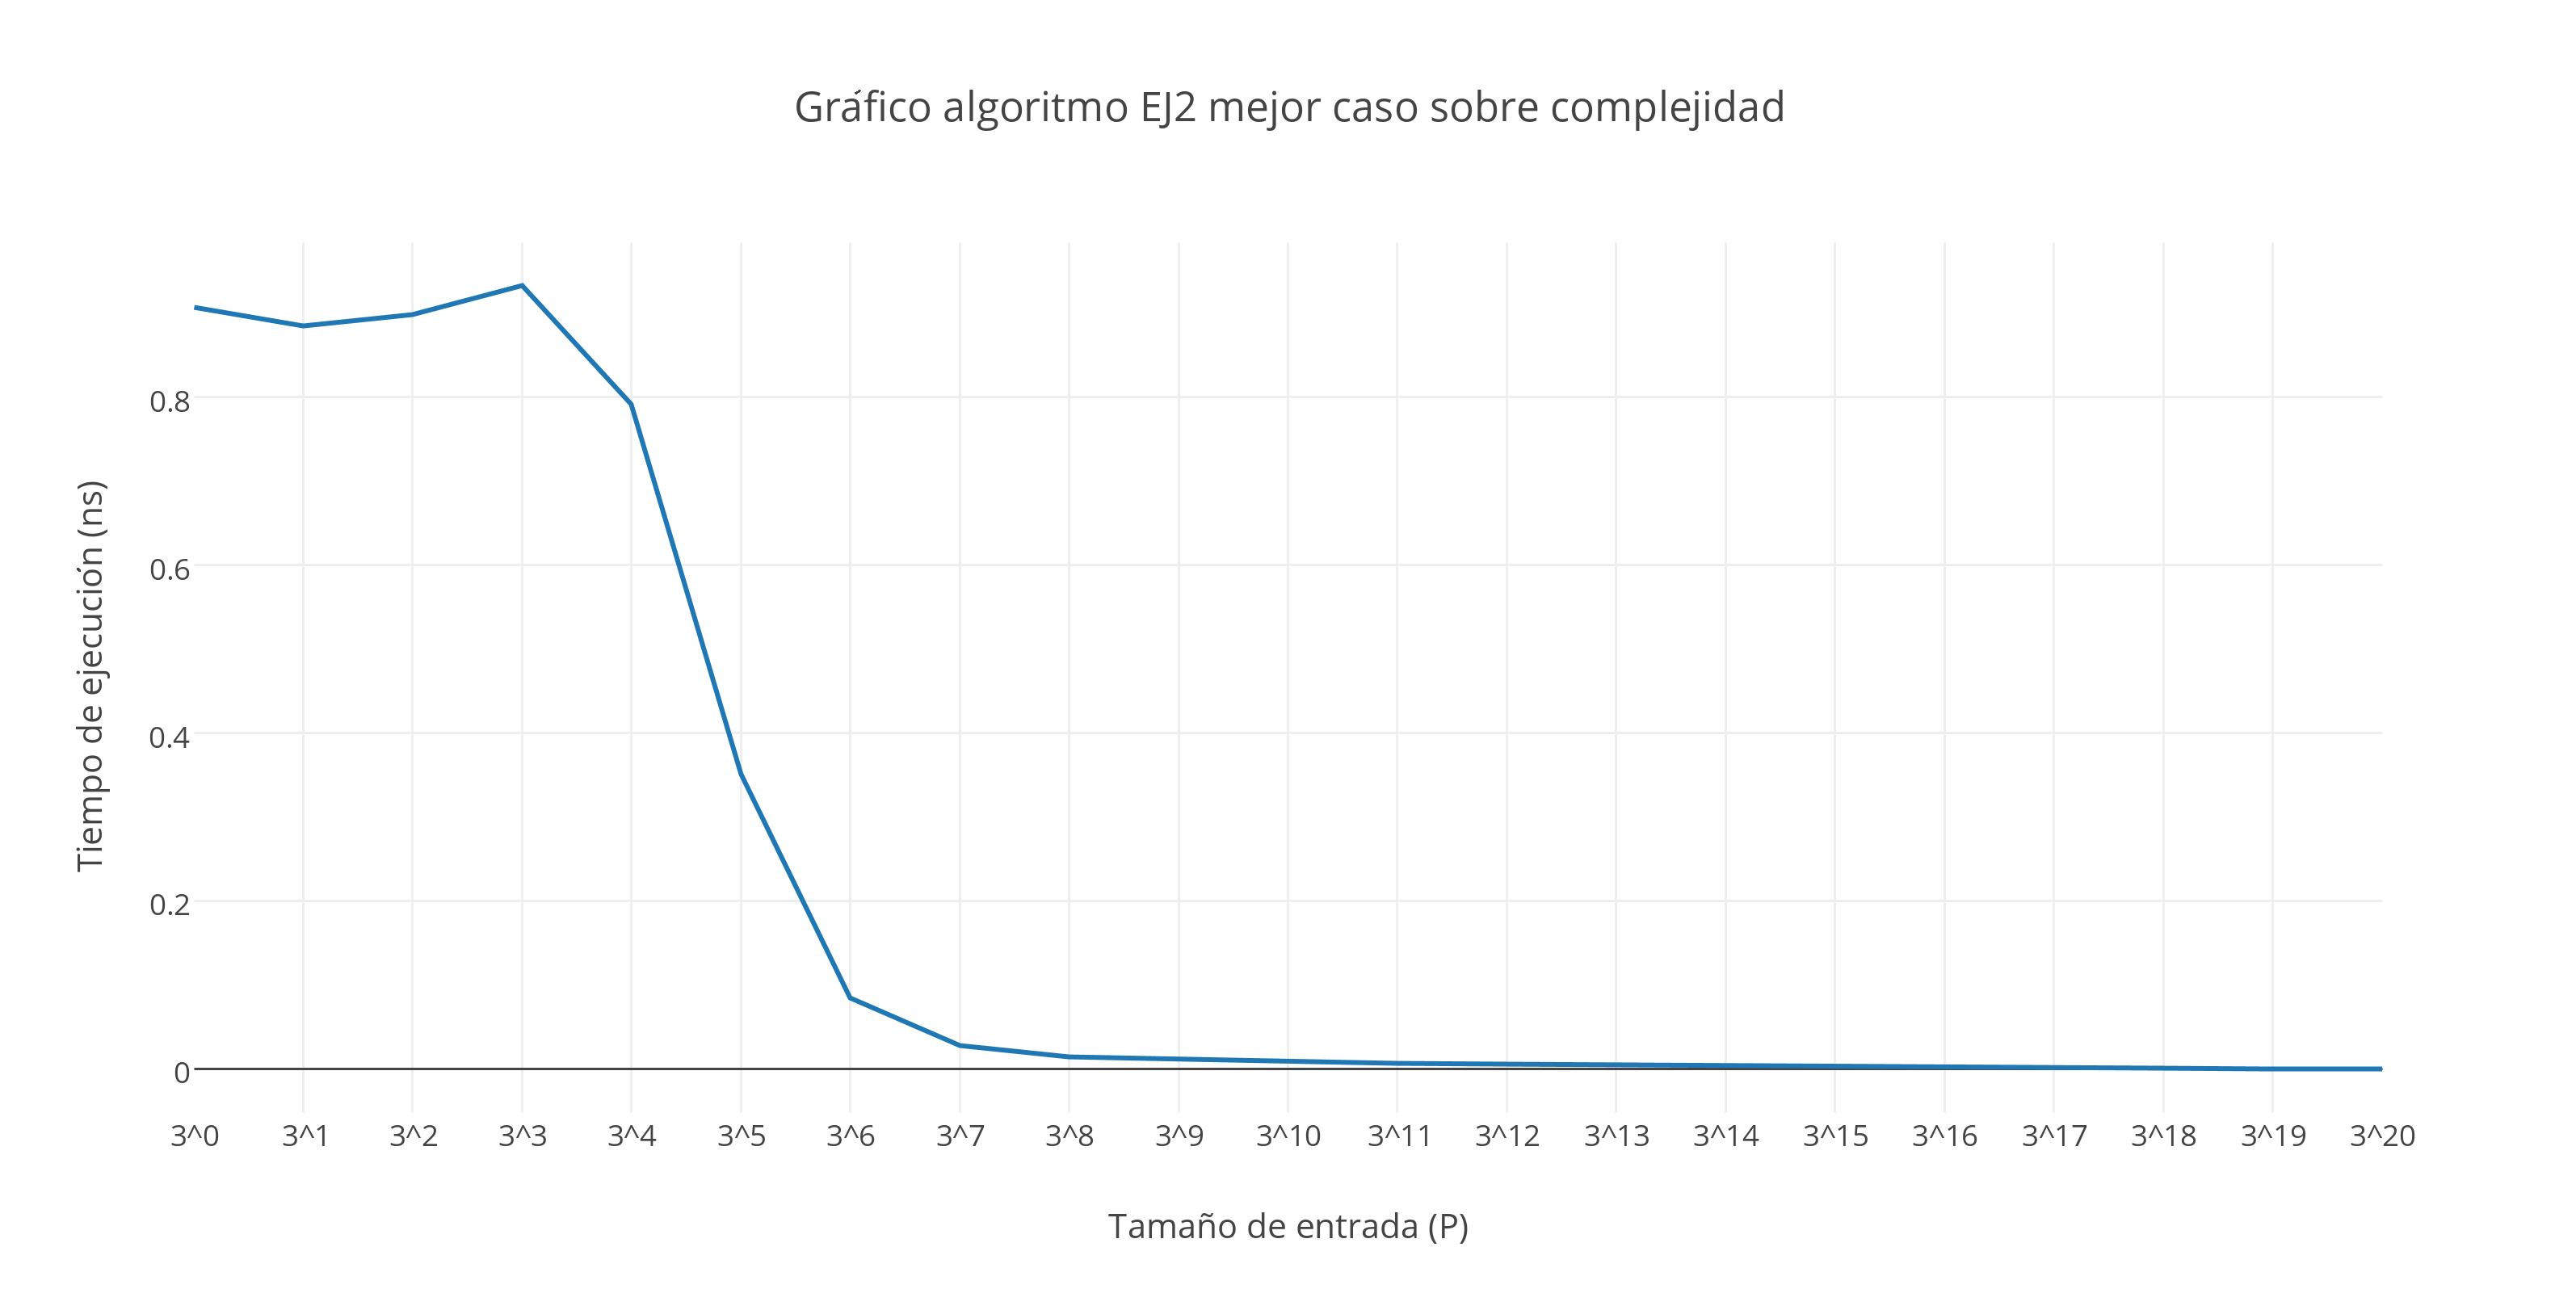
\includegraphics[scale=0.65]{./EJ2/mejorcaso1.png}
{$Gr$\'a$fico$ \ 1.4 - $Mejor Caso / Complejidad$ $O()$}
  \end{center}
  \vspace*{0.3cm}


Para realizar esta experimentaci\'on nos parecio prudente, realizar un promedio con el mismo input de aproximadamente 20 corridas
tanto para la complejidad como para nuestro algoritmo y una vez calculado dicho promedio de ambas cosas realizamos la divisi\'on para
obtener resultados m\'as relevantes.\\ 

%Se puede observar en el gr\'afico 2.4, como luego de realizar la divisi\'on por la complejidad cuando el n aumenta el valor tiende a 0, tomando un valor m\'aximo en 0.93. Y, en el gr\'afico 2.4 se ve como la funci\'on resultante tiene picos en los cuales llega a un m\'aximo igual a 1 y cuando el valor de entrada aumenta la funci\'on tiende a 0.5. Por lo tanto, podemos concluir que para el mejor caso nuestro algoritmo se encuentra considerablemente por debajo de la cota teorica $O(\sqrt{P})$ y asintotizado por la cota $O(log(P))$\\

Luego, para verificar el peor caso, desarrollamos otro gr\'afico de mediciones como enunciamos al principio el cual contendr\'a los peor casos posibles para nuestro algoritmo. Como dichos casos presentan las mismas entradas v\'alidas tanto en uno como en otro, fue posible graficarlos juntos mostrando el tiempo medido para cada entrada.\\

 \vspace*{0.3cm} \vspace*{0.3cm}
  \begin{center}
 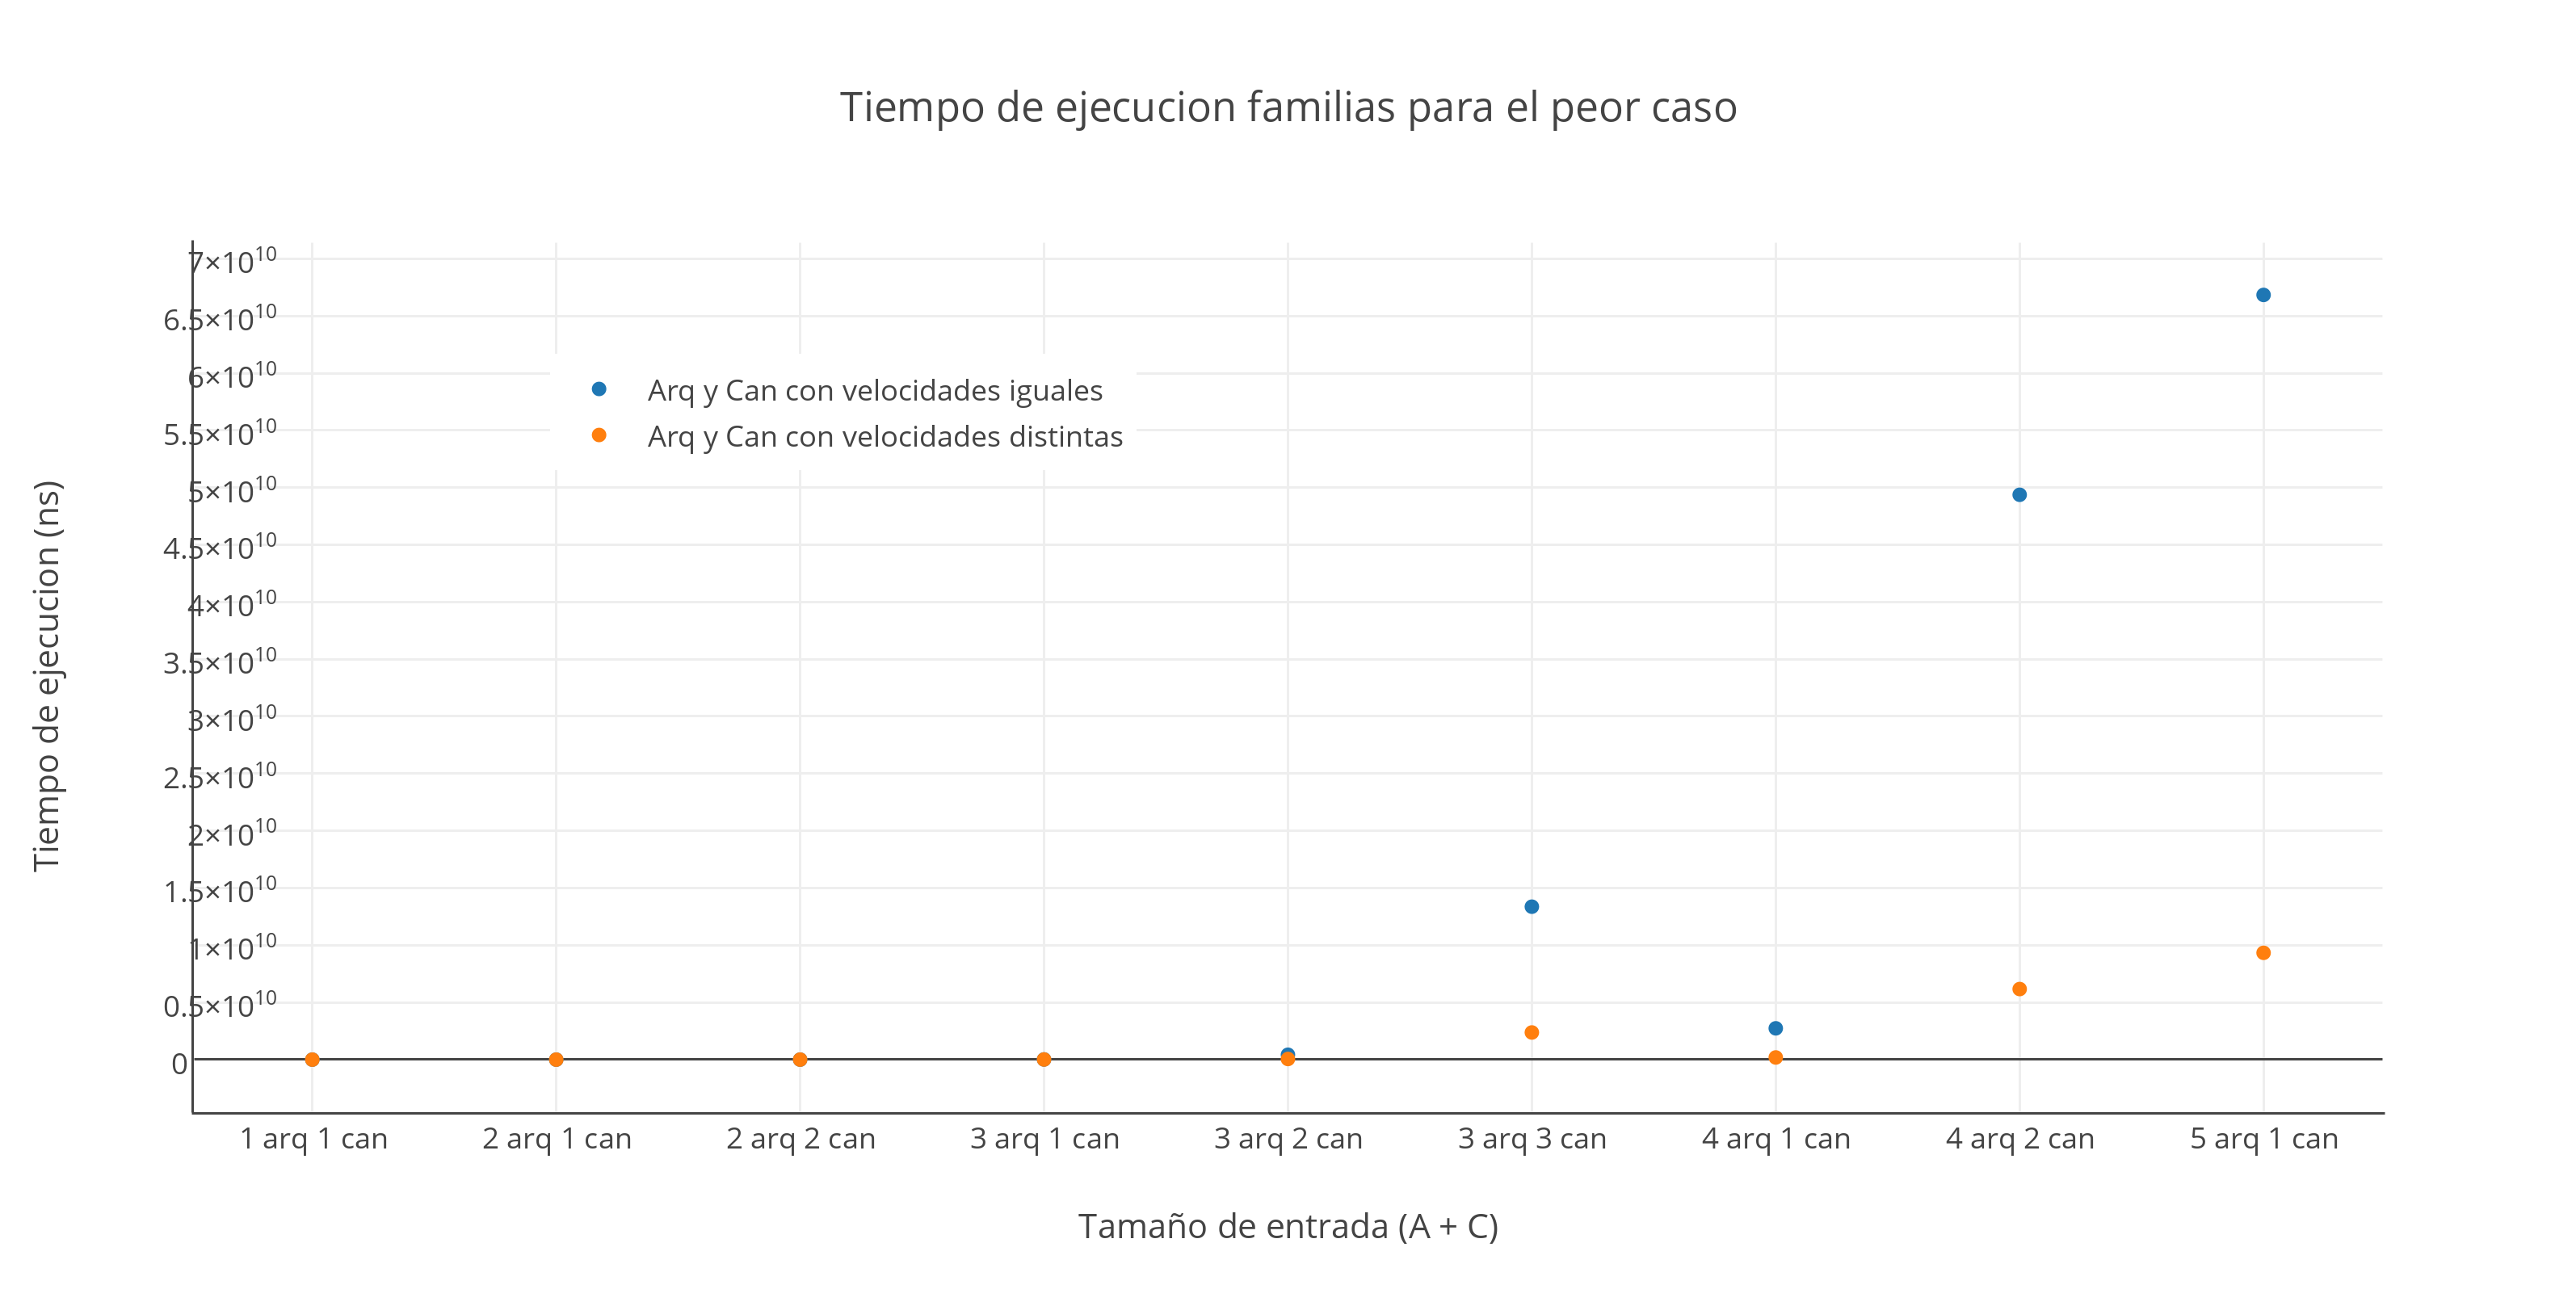
\includegraphics[scale=0.65]{./EJ1/comparativopeorcaso.png}
 {$Gr$\'a$fico$ \ 1.6 - $Comparativo$ $Peor$ $Caso$}
  \end{center}
  \vspace*{0.3cm}

Se puede observar en el gr\'afico, dos funciones las cuales representan el tiempo de ejecuci\'on de las familias que resultan menos beneficiadas a la hora de trabajar con nuestro algoritmo:\\
\begin{itemize}
\item Todos los canibales y arqueologos presentan velocidades iguales
\item Todos los canibales y arqueologos presentan velocidades distintas
\end{itemize}

Es posible observar en el gr\'afico que la funci\'on representativa de la flia n\'umero 1, presenta una peor performance en relaci\'on a la otra. Esto se debe a que nuestro algoritmo va chequeando y probando todos las permutaciones posibles de pares que viajen de un lado al otro, y, adem\'as como el mismo tiene realizado una poda la cual consiste en anular las ramas que tarden m\'as tiempo, dicha familia finalizar\'a m\'as tarde su ejecuci\'on en relaci\'on a la otra ya que al tener a todas las personas con las mismas velocidades dicha poda no podr\'a ser utilizada, generando de esta forma, el peor caso posible para nuestro algoritmo.

Por lo tanto, el peor caso para nuestro algoritmo ser\'a cuando \textbf{Todos los canibales y arqueologos presentan velocidades iguales, y dicha combinaci\'on de arqueologo - canibal tenga una soluci\'on posible}


\vspace*{0.3cm} \vspace*{0.3cm}
  \begin{center}
 %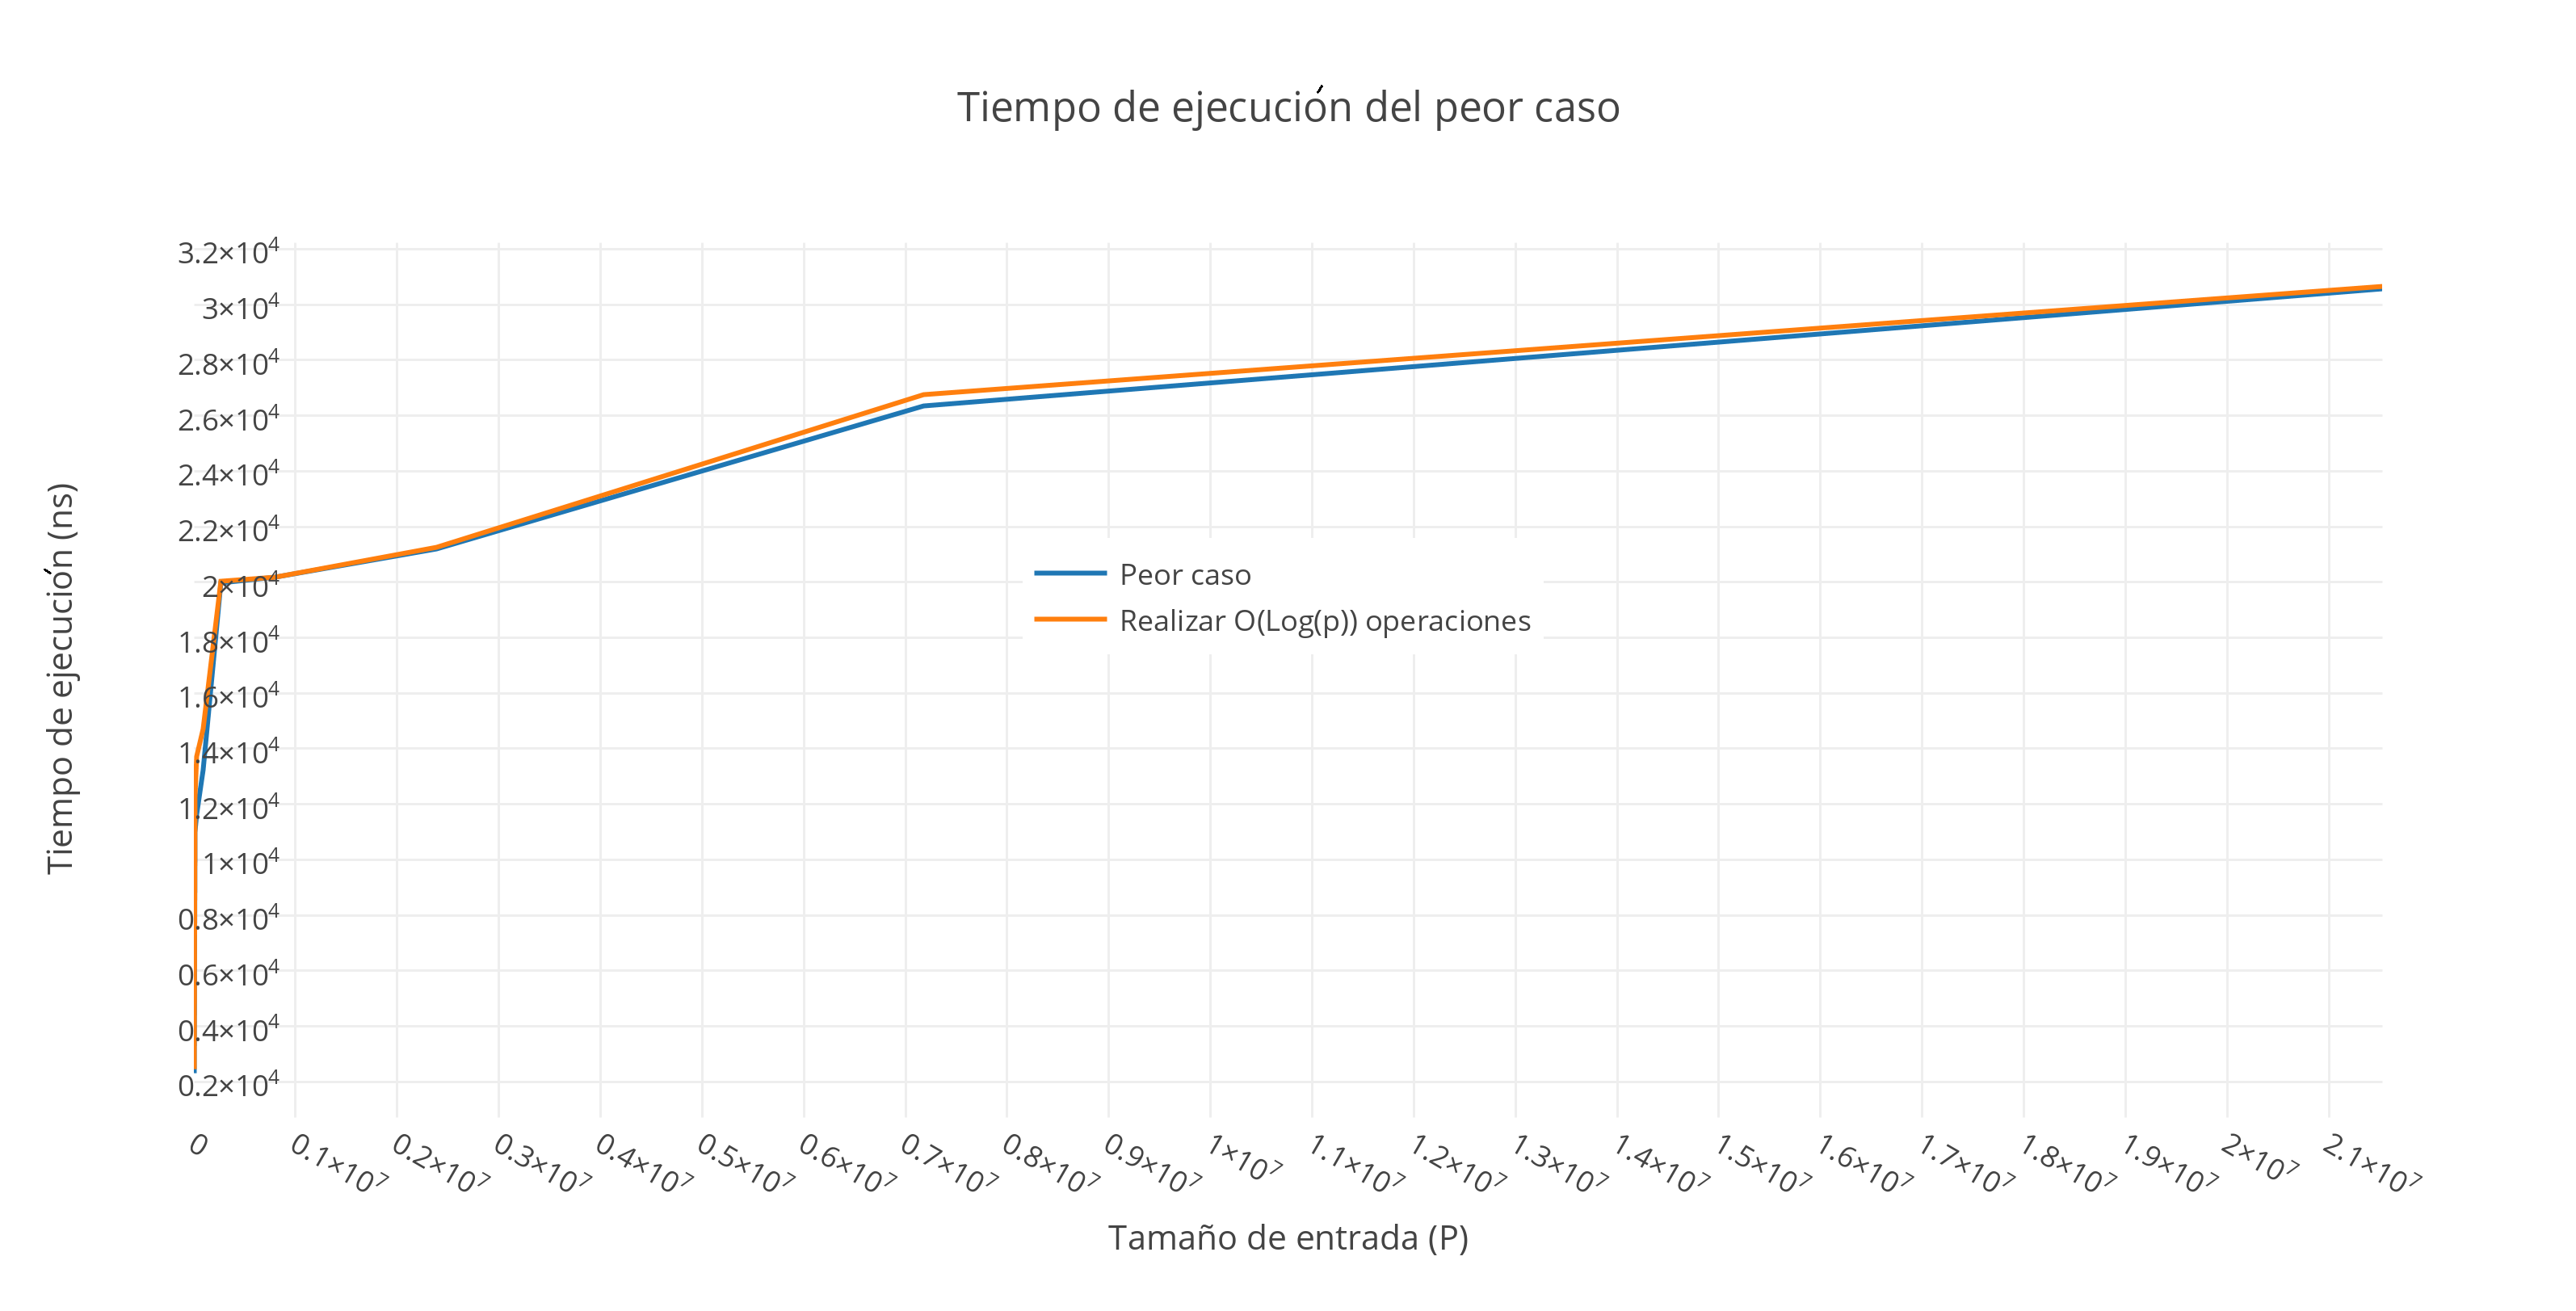
\includegraphics[scale=0.65]{./EJ2/peorcaso1.png}
 {$Gr$\'a$fico$ \ 1.6 - $Peor Caso$}
  \end{center}
  \vspace*{0.3cm}

Dividiendo por la complejidad propuesta llegamos a:\\

\vspace*{0.3cm} \vspace*{0.3cm}
  \begin{center}
 %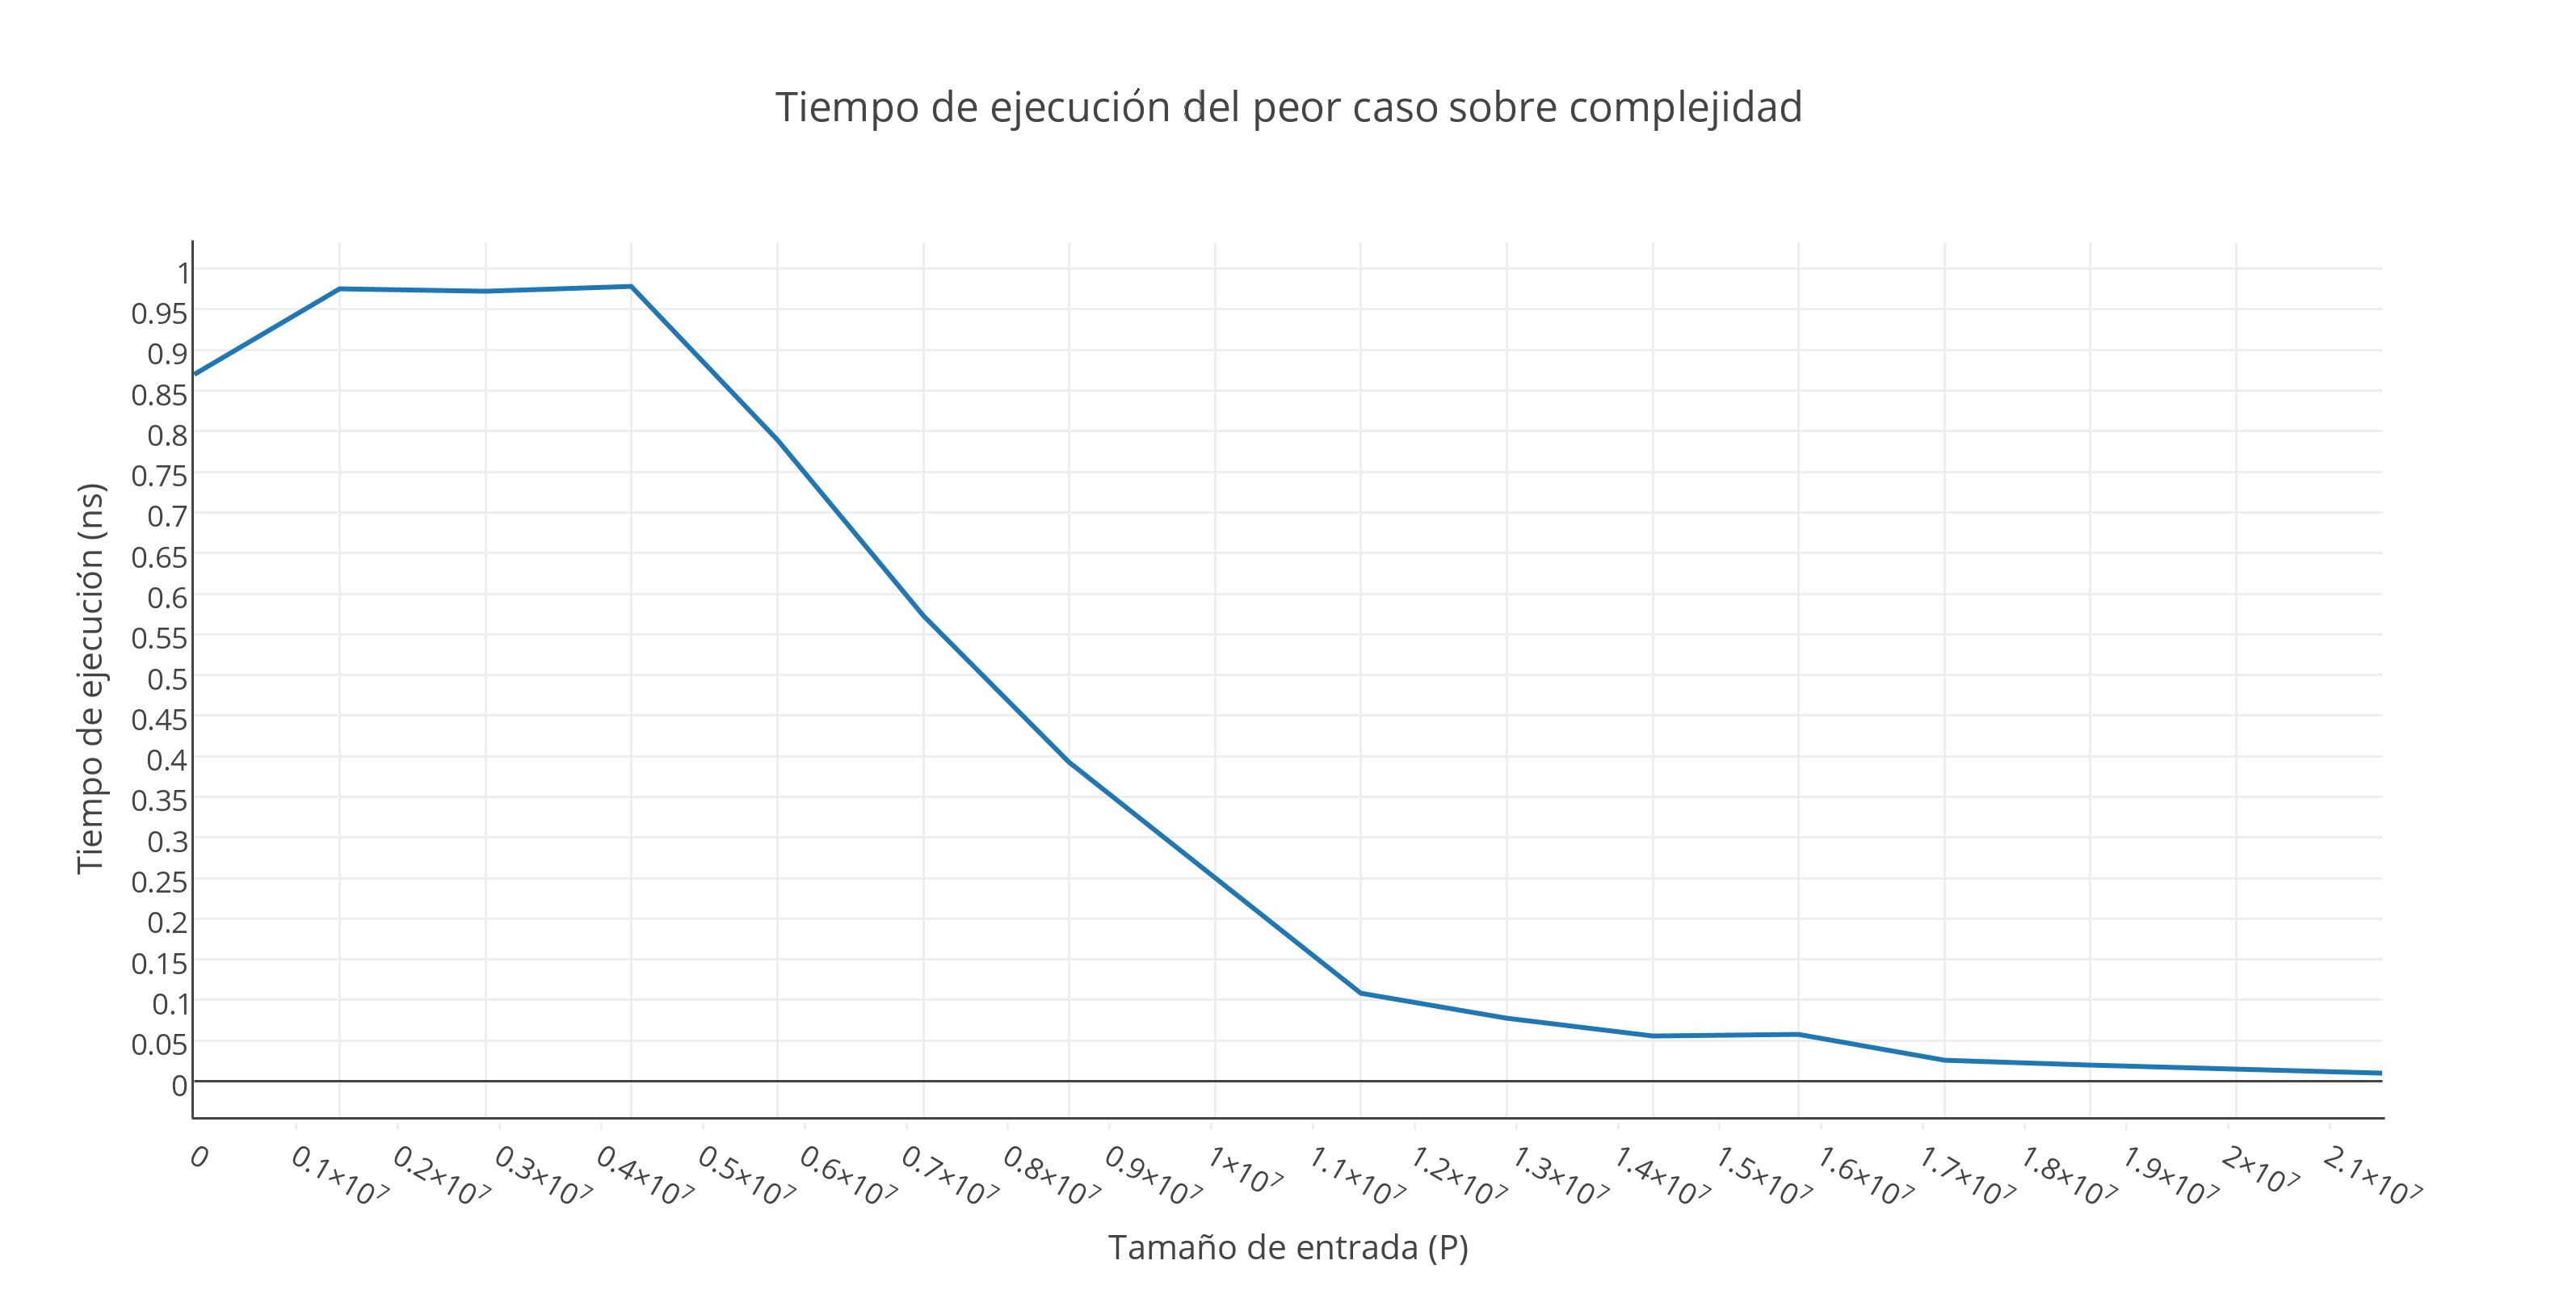
\includegraphics[scale=0.65]{./EJ2/peorcaso2.png}
 {$Gr$\'a$fico$ \ 1.7 - $Peor Caso / Complejidad$ $O()$}
  \end{center}
  \vspace*{0.3cm}

Para realizar esta experimentaci\'on nos parecio acorde, realizar un promedio con el mismo input de aproximadamente 20 corridas
tanto para la complejidad como para nuestro algoritmo y una vez calculado dicho promedio de ambas cosas realizamos la divisi\'on para
obtener resultados m\'as relevantes.\\ 

%Como se puede observar en el gr\'afico 2.6 y  2.7, la funci\'on resultante de nuestro algoritmo es considerablemente mejor que la de la cota teorica $O(\sqrt{P})$ y presenta un tiempo similar al de la funci\'on resultante de la cota $O(log(P))$. Al igual que en el mejor caso, se gr\'aficaron las primeras instancias para que el gr\'afico pueda ser m\'as legible.
%Luego, en el gr\'afico 2.8 a pesar de tardar varios nanosegundos m\'as que en el mejor caso, al dividir por la complejidad teorica
%la función resultante tambi\'en tiende a 0 quedando comparativamente por encima del mejor caso.\\



Luego de dichos experimentos y casos probados, se puede concluir que a pesar de utilizar todas las pesas como en el peor caso nos mantenemos dentro de la complejidad propuesta como hab\'iamos mostrado en nuestro desarrollo de la complejidad.\\
